% Options for packages loaded elsewhere
\PassOptionsToPackage{unicode}{hyperref}
\PassOptionsToPackage{hyphens}{url}
%
\documentclass[
]{book}
\title{Fundamentals of Mathematics and Statistics with R}
\author{Dr.~Priyanga D. Talagala}
\date{2023-03-30}

\usepackage{amsmath,amssymb}
\usepackage{lmodern}
\usepackage{iftex}
\ifPDFTeX
  \usepackage[T1]{fontenc}
  \usepackage[utf8]{inputenc}
  \usepackage{textcomp} % provide euro and other symbols
\else % if luatex or xetex
  \usepackage{unicode-math}
  \defaultfontfeatures{Scale=MatchLowercase}
  \defaultfontfeatures[\rmfamily]{Ligatures=TeX,Scale=1}
\fi
% Use upquote if available, for straight quotes in verbatim environments
\IfFileExists{upquote.sty}{\usepackage{upquote}}{}
\IfFileExists{microtype.sty}{% use microtype if available
  \usepackage[]{microtype}
  \UseMicrotypeSet[protrusion]{basicmath} % disable protrusion for tt fonts
}{}
\makeatletter
\@ifundefined{KOMAClassName}{% if non-KOMA class
  \IfFileExists{parskip.sty}{%
    \usepackage{parskip}
  }{% else
    \setlength{\parindent}{0pt}
    \setlength{\parskip}{6pt plus 2pt minus 1pt}}
}{% if KOMA class
  \KOMAoptions{parskip=half}}
\makeatother
\usepackage{xcolor}
\usepackage{color}
\usepackage{fancyvrb}
\newcommand{\VerbBar}{|}
\newcommand{\VERB}{\Verb[commandchars=\\\{\}]}
\DefineVerbatimEnvironment{Highlighting}{Verbatim}{commandchars=\\\{\}}
% Add ',fontsize=\small' for more characters per line
\usepackage{framed}
\definecolor{shadecolor}{RGB}{248,248,248}
\newenvironment{Shaded}{\begin{snugshade}}{\end{snugshade}}
\newcommand{\AlertTok}[1]{\textcolor[rgb]{0.94,0.16,0.16}{#1}}
\newcommand{\AnnotationTok}[1]{\textcolor[rgb]{0.56,0.35,0.01}{\textbf{\textit{#1}}}}
\newcommand{\AttributeTok}[1]{\textcolor[rgb]{0.77,0.63,0.00}{#1}}
\newcommand{\BaseNTok}[1]{\textcolor[rgb]{0.00,0.00,0.81}{#1}}
\newcommand{\BuiltInTok}[1]{#1}
\newcommand{\CharTok}[1]{\textcolor[rgb]{0.31,0.60,0.02}{#1}}
\newcommand{\CommentTok}[1]{\textcolor[rgb]{0.56,0.35,0.01}{\textit{#1}}}
\newcommand{\CommentVarTok}[1]{\textcolor[rgb]{0.56,0.35,0.01}{\textbf{\textit{#1}}}}
\newcommand{\ConstantTok}[1]{\textcolor[rgb]{0.00,0.00,0.00}{#1}}
\newcommand{\ControlFlowTok}[1]{\textcolor[rgb]{0.13,0.29,0.53}{\textbf{#1}}}
\newcommand{\DataTypeTok}[1]{\textcolor[rgb]{0.13,0.29,0.53}{#1}}
\newcommand{\DecValTok}[1]{\textcolor[rgb]{0.00,0.00,0.81}{#1}}
\newcommand{\DocumentationTok}[1]{\textcolor[rgb]{0.56,0.35,0.01}{\textbf{\textit{#1}}}}
\newcommand{\ErrorTok}[1]{\textcolor[rgb]{0.64,0.00,0.00}{\textbf{#1}}}
\newcommand{\ExtensionTok}[1]{#1}
\newcommand{\FloatTok}[1]{\textcolor[rgb]{0.00,0.00,0.81}{#1}}
\newcommand{\FunctionTok}[1]{\textcolor[rgb]{0.00,0.00,0.00}{#1}}
\newcommand{\ImportTok}[1]{#1}
\newcommand{\InformationTok}[1]{\textcolor[rgb]{0.56,0.35,0.01}{\textbf{\textit{#1}}}}
\newcommand{\KeywordTok}[1]{\textcolor[rgb]{0.13,0.29,0.53}{\textbf{#1}}}
\newcommand{\NormalTok}[1]{#1}
\newcommand{\OperatorTok}[1]{\textcolor[rgb]{0.81,0.36,0.00}{\textbf{#1}}}
\newcommand{\OtherTok}[1]{\textcolor[rgb]{0.56,0.35,0.01}{#1}}
\newcommand{\PreprocessorTok}[1]{\textcolor[rgb]{0.56,0.35,0.01}{\textit{#1}}}
\newcommand{\RegionMarkerTok}[1]{#1}
\newcommand{\SpecialCharTok}[1]{\textcolor[rgb]{0.00,0.00,0.00}{#1}}
\newcommand{\SpecialStringTok}[1]{\textcolor[rgb]{0.31,0.60,0.02}{#1}}
\newcommand{\StringTok}[1]{\textcolor[rgb]{0.31,0.60,0.02}{#1}}
\newcommand{\VariableTok}[1]{\textcolor[rgb]{0.00,0.00,0.00}{#1}}
\newcommand{\VerbatimStringTok}[1]{\textcolor[rgb]{0.31,0.60,0.02}{#1}}
\newcommand{\WarningTok}[1]{\textcolor[rgb]{0.56,0.35,0.01}{\textbf{\textit{#1}}}}
\usepackage{longtable,booktabs,array}
\usepackage{calc} % for calculating minipage widths
% Correct order of tables after \paragraph or \subparagraph
\usepackage{etoolbox}
\makeatletter
\patchcmd\longtable{\par}{\if@noskipsec\mbox{}\fi\par}{}{}
\makeatother
% Allow footnotes in longtable head/foot
\IfFileExists{footnotehyper.sty}{\usepackage{footnotehyper}}{\usepackage{footnote}}
\makesavenoteenv{longtable}
\usepackage{graphicx}
\makeatletter
\def\maxwidth{\ifdim\Gin@nat@width>\linewidth\linewidth\else\Gin@nat@width\fi}
\def\maxheight{\ifdim\Gin@nat@height>\textheight\textheight\else\Gin@nat@height\fi}
\makeatother
% Scale images if necessary, so that they will not overflow the page
% margins by default, and it is still possible to overwrite the defaults
% using explicit options in \includegraphics[width, height, ...]{}
\setkeys{Gin}{width=\maxwidth,height=\maxheight,keepaspectratio}
% Set default figure placement to htbp
\makeatletter
\def\fps@figure{htbp}
\makeatother
\setlength{\emergencystretch}{3em} % prevent overfull lines
\providecommand{\tightlist}{%
  \setlength{\itemsep}{0pt}\setlength{\parskip}{0pt}}
\setcounter{secnumdepth}{5}
\usepackage{booktabs}
\usepackage{amsthm}
\makeatletter
\def\thm@space@setup{%
  \thm@preskip=8pt plus 2pt minus 4pt
  \thm@postskip=\thm@preskip
}
\makeatother
\usepackage{fancyhdr}
\pagestyle{fancy}
\fancyfoot[CO,CE]{Prepared by Dr. Priyanga D. Talagala  (Copyright 2023 P. D. Talagala)}
\fancyfoot[LE,RO]{\thepage}
\usepackage{wrapfig}
\usepackage{floatrow}
\floatplacement{figure}{H}
\floatplacement{table}{H}
\makeatletter\renewcommand*{\fps@figure}{H}\makeatother
\ifLuaTeX
  \usepackage{selnolig}  % disable illegal ligatures
\fi
\usepackage[]{natbib}
\bibliographystyle{apalike}
\IfFileExists{bookmark.sty}{\usepackage{bookmark}}{\usepackage{hyperref}}
\IfFileExists{xurl.sty}{\usepackage{xurl}}{} % add URL line breaks if available
\urlstyle{same} % disable monospaced font for URLs
\hypersetup{
  pdftitle={Fundamentals of Mathematics and Statistics with R},
  pdfauthor={Dr.~Priyanga D. Talagala},
  hidelinks,
  pdfcreator={LaTeX via pandoc}}

<<<<<<< HEAD
=======
\title{Fundamentals of Mathematics and Statistics with R}
\author{Dr.~Priyanga D. Talagala}
\date{2023-01-14}

>>>>>>> db2d36962e520f9ed1862fd4eb2c519e8da84f67
\begin{document}
\maketitle

{
\setcounter{tocdepth}{1}
\tableofcontents
}
\hypertarget{intro}{%
\chapter{Introduction to R}\label{intro}}

\pagenumbering{arabic}

\hypertarget{installing-r}{%
\section{Installing R}\label{installing-r}}

\begin{itemize}
\item
<<<<<<< HEAD
  \textbf{Step 1:} First download R freely from the Comprehensive R Archive Network (CRAN) \url{https://posit.co/download/rstudio-desktop/}.
  (At the moment of writing, R 4.2.3 is the latest version. Choose the most recent one.)
=======
  \textbf{Step 1:} First download R freely from the Comprehensive R Archive Network (CRAN) \url{https://cran.r-project.org/}.
  (At the moment of writing, R 4.2.2 is the latest version. Choose the most recent one.)
>>>>>>> db2d36962e520f9ed1862fd4eb2c519e8da84f67
\item
  \textbf{Step 2:} Then install R Studio's IDE (stands for integrated development environment), a powerful user interface for R from \url{https://posit.co/download/rstudio-desktop/}. Get the Open Source Edition of RStudio Desktop. RStudio allows you to run R in a more user-friendly environment.

  \begin{itemize}
  \item
    You need to install \textbf{both} R and Rstudio to use RStudio.
  \item
    If you have a pre-existing installation of R and/or RStudio, I highly recommend that you re install both and get as current as possible.
  \end{itemize}
\item
  \textbf{Step 3:} Then open \textbf{Rstudio}.
\end{itemize}

\hypertarget{rstudio-layout}{%
\section{RStudio layout}\label{rstudio-layout}}

The RStudio interface consists of four windows (see Figure 1 and 2).

\begin{enumerate}
\def\labelenumi{\arabic{enumi}.}
\item
  Bottom left: console window (also called command window). \textbf{This is where you type and run all your R commands}
\item
  Top left: editor window (also called script window).
\item
  Top right: workspace / history window.
\item
  Bottom right: Files / plots / packages / help window.
\end{enumerate}

\begin{center}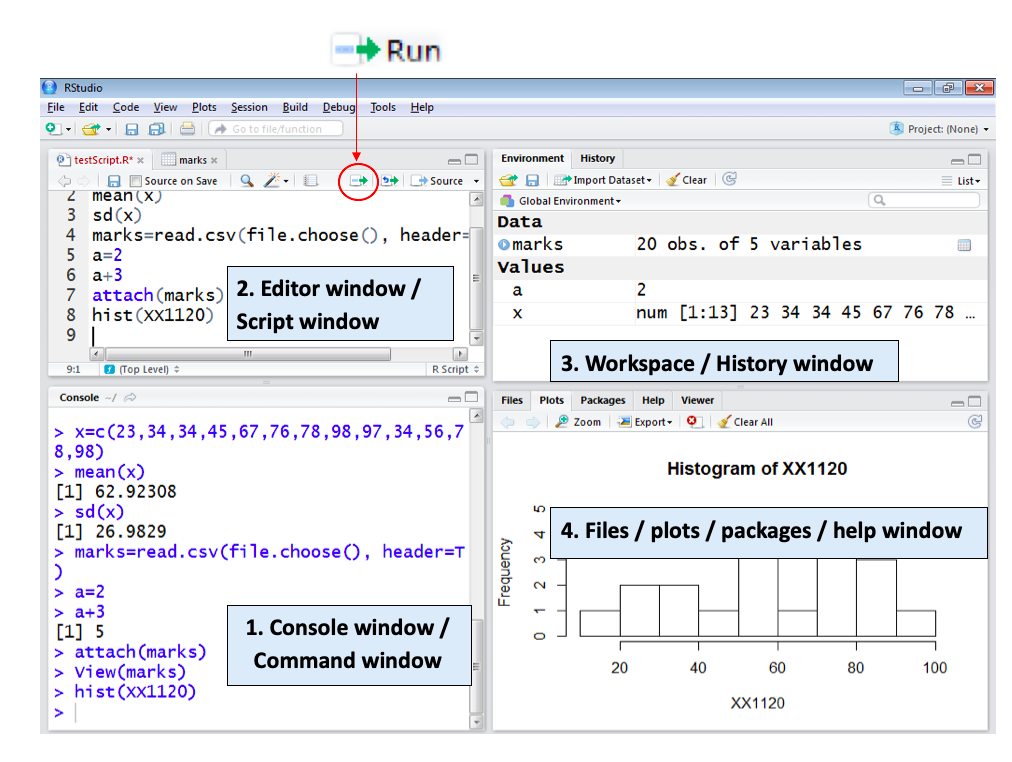
\includegraphics[width=1\linewidth]{figure/Rstudio1} \end{center}

\begin{center}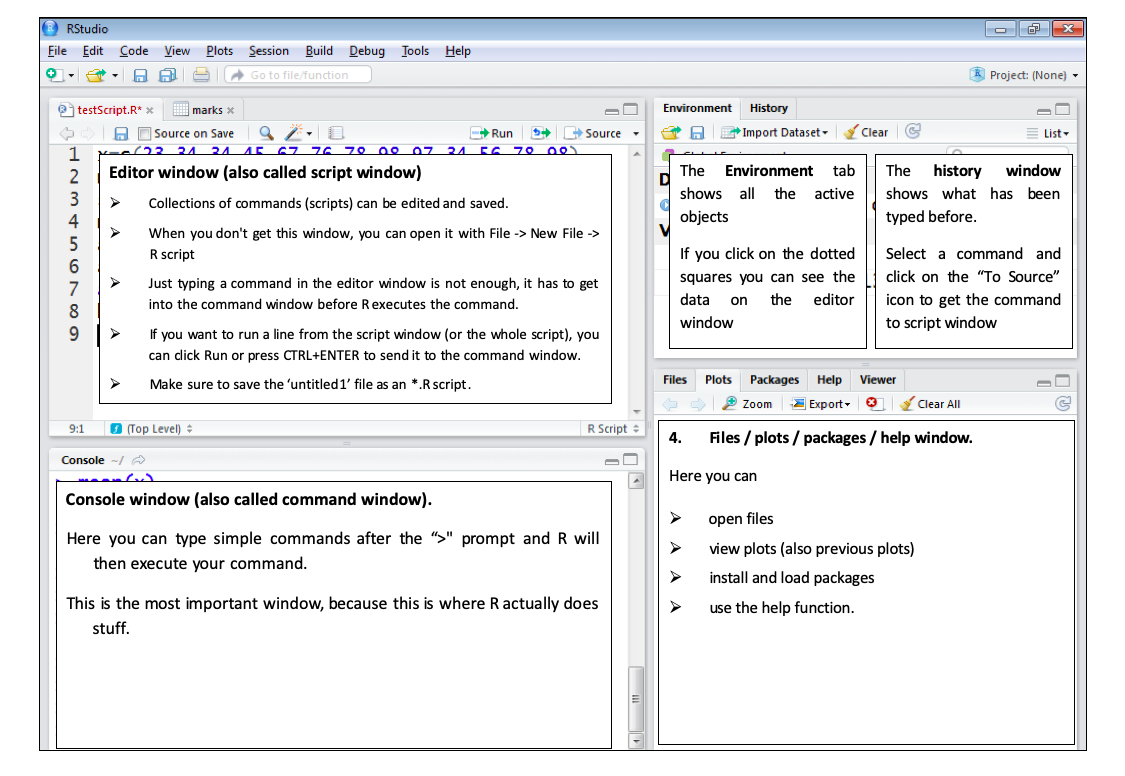
\includegraphics[width=1\linewidth]{figure/Rstudio2} \end{center}

Now you are familiar with the layout. Let's begin with R basics.

\hypertarget{installing-an-r-package}{%
\section{Installing an R Package}\label{installing-an-r-package}}

\begin{itemize}
\item
  The primary location for obtaining R packages is CRAN
\item
  Packages can be installed with the \texttt{install.packages()} function in R
\item
  To install a single package, pass the name of the package to the \texttt{install.packages()} function as the first argument
\end{itemize}

The following the code installs the \texttt{tidyverse} package from CRAN

\begin{Shaded}
\begin{Highlighting}[]
\FunctionTok{install.packages}\NormalTok{(}\StringTok{"tidyverse"}\NormalTok{)}
\end{Highlighting}
\end{Shaded}

\begin{itemize}
\item
  This command downloads the \texttt{tidyverse} package from CRAN and installs it on your computer
\item
  Any packages on which this package depends will also be downloaded and installed
\item
  \textbf{Installing the tidyverse package could take several minutes. You only need to do this once}.
\end{itemize}

\hypertarget{loading-an-r-packages}{%
\section{Loading an R Packages}\label{loading-an-r-packages}}

\begin{itemize}
\item
  Installing a package does not make it immediately available to you in R; you must load the package
\item
  The \texttt{library()} function is used to load packages into R
\item
  The following code is used to load the tidyverse package into R
\item
  \textbf{NOTE:} Do not put the package name in quotes!
\end{itemize}

\begin{Shaded}
\begin{Highlighting}[]
\FunctionTok{library}\NormalTok{(tidyverse)}
\end{Highlighting}
\end{Shaded}

\begin{verbatim}
<<<<<<< HEAD
## -- Attaching packages --------------------------------------- tidyverse 1.3.1 --
\end{verbatim}

\begin{verbatim}
## v ggplot2 3.3.6      v purrr   0.3.5 
## v tibble  3.1.8      v dplyr   1.0.10
## v tidyr   1.2.0      v stringr 1.4.1 
## v readr   2.1.2      v forcats 0.5.1
\end{verbatim}

\begin{verbatim}
=======
## -- Attaching packages --------------------------------------- tidyverse 1.3.2 --
## v ggplot2 3.4.0      v purrr   1.0.1 
## v tibble  3.1.8      v dplyr   1.0.10
## v tidyr   1.2.1      v stringr 1.4.1 
## v readr   2.1.3      v forcats 0.5.2 
>>>>>>> db2d36962e520f9ed1862fd4eb2c519e8da84f67
## -- Conflicts ------------------------------------------ tidyverse_conflicts() --
## x dplyr::filter() masks stats::filter()
## x dplyr::lag()    masks stats::lag()
\end{verbatim}

\begin{itemize}
\tightlist
\item
  Some packages produce messages when they are loaded (but some don't)
\end{itemize}

\hypertarget{getting-started-with-r}{%
\section{Getting started with R}\label{getting-started-with-r}}

\href{https://cran.r-project.org/doc/manuals/R-intro.pdf}{An Introduction to R: https://cran.r-project.org/doc/manuals/R-intro.pdf}

\hypertarget{differentiation}{%
\chapter{Differentiation}\label{differentiation}}

First, we take the equation as an expression

\begin{Shaded}
\begin{Highlighting}[]
\NormalTok{f }\OtherTok{\textless{}{-}} \FunctionTok{expression}\NormalTok{(x}\SpecialCharTok{\^{}}\DecValTok{2}\NormalTok{)}
\end{Highlighting}
\end{Shaded}

To calculate first derivative of \(f\), we use \texttt{D()} function and \texttt{x} to specify that derivation has to be carried out with respect to
\(x\).

\begin{Shaded}
\begin{Highlighting}[]
\NormalTok{f\_1 }\OtherTok{\textless{}{-}} \FunctionTok{D}\NormalTok{(f, }\StringTok{"x"}\NormalTok{)}
\FunctionTok{print}\NormalTok{(f\_1)}
\end{Highlighting}
\end{Shaded}

\begin{verbatim}
## 2 * x
\end{verbatim}

Sketch the graph of \(f\) and \(f^\prime\)

\begin{Shaded}
\begin{Highlighting}[]
\FunctionTok{library}\NormalTok{(ggplot2)}
\NormalTok{x }\OtherTok{\textless{}{-}} \FunctionTok{seq}\NormalTok{(}\SpecialCharTok{{-}}\DecValTok{1}\NormalTok{, }\DecValTok{1}\NormalTok{, }\AttributeTok{by =} \FloatTok{0.1}\NormalTok{)}
\NormalTok{y }\OtherTok{\textless{}{-}} \FunctionTok{eval}\NormalTok{(f)}
\NormalTok{x }\OtherTok{\textless{}{-}} \FunctionTok{seq}\NormalTok{(}\SpecialCharTok{{-}}\DecValTok{1}\NormalTok{, }\DecValTok{1}\NormalTok{, }\AttributeTok{by =} \FloatTok{0.1}\NormalTok{)}
\NormalTok{y1 }\OtherTok{\textless{}{-}} \FunctionTok{eval}\NormalTok{(f\_1)}
\NormalTok{data }\OtherTok{\textless{}{-}} \FunctionTok{data.frame}\NormalTok{(x, y, y1)}
\FunctionTok{head}\NormalTok{(data)}
\end{Highlighting}
\end{Shaded}

\begin{verbatim}
##      x    y   y1
## 1 -1.0 1.00 -2.0
## 2 -0.9 0.81 -1.8
## 3 -0.8 0.64 -1.6
## 4 -0.7 0.49 -1.4
## 5 -0.6 0.36 -1.2
## 6 -0.5 0.25 -1.0
\end{verbatim}

\begin{Shaded}
\begin{Highlighting}[]
\NormalTok{p }\OtherTok{\textless{}{-}} \FunctionTok{ggplot}\NormalTok{(data, }\FunctionTok{aes}\NormalTok{(}\AttributeTok{x =}\NormalTok{ x, }\AttributeTok{y =}\NormalTok{ y)) }\SpecialCharTok{+}
  \FunctionTok{geom\_line}\NormalTok{()}
\FunctionTok{print}\NormalTok{(p)}
\end{Highlighting}
\end{Shaded}

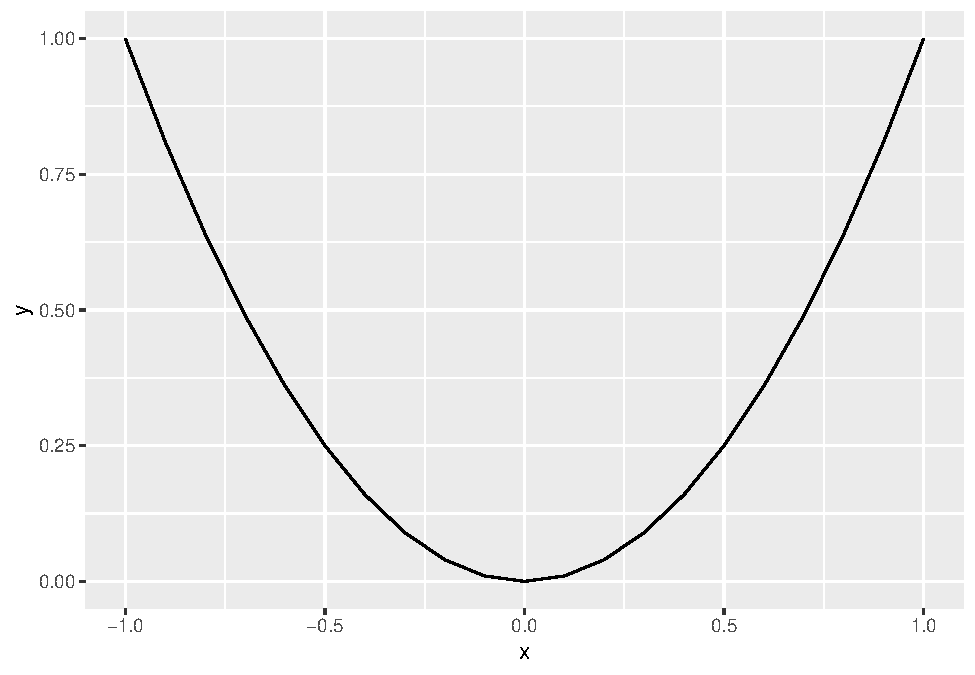
\includegraphics{bookdown-demo_files/figure-latex/unnamed-chunk-7-1.pdf}

\begin{Shaded}
\begin{Highlighting}[]
\NormalTok{q }\OtherTok{\textless{}{-}} \FunctionTok{ggplot}\NormalTok{(data, }\FunctionTok{aes}\NormalTok{(}\AttributeTok{x =}\NormalTok{ x, }\AttributeTok{y =}\NormalTok{ y1)) }\SpecialCharTok{+}
  \FunctionTok{geom\_line}\NormalTok{()}
\FunctionTok{print}\NormalTok{(q)}
\end{Highlighting}
\end{Shaded}

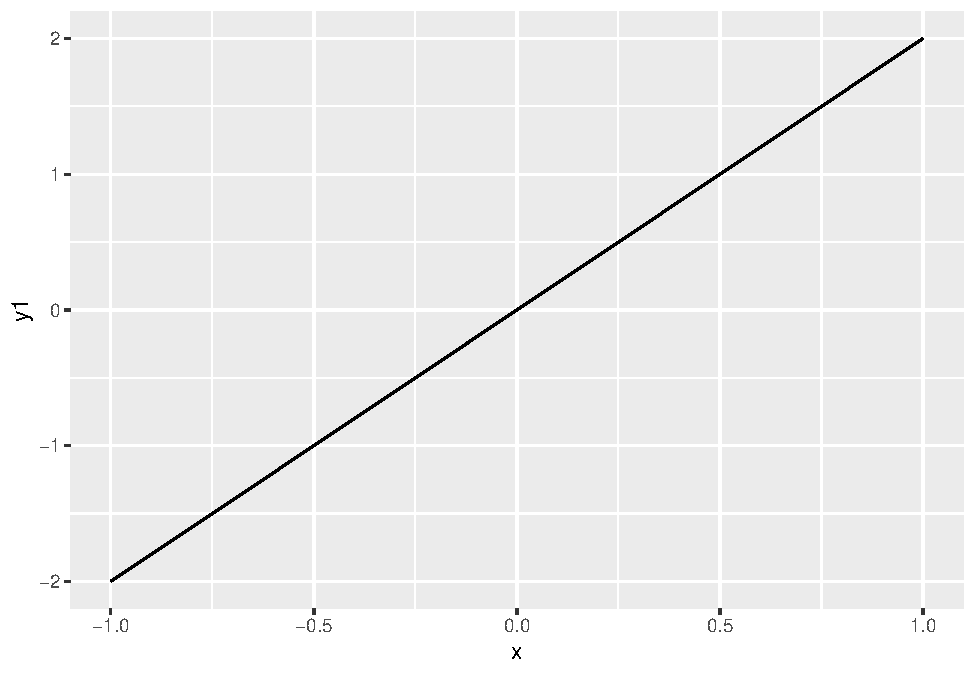
\includegraphics{bookdown-demo_files/figure-latex/unnamed-chunk-8-1.pdf}

\hypertarget{higher-derivatives}{%
\section{Higher Derivatives}\label{higher-derivatives}}

The following R command can be used to find second derivative of the above \(f\).

\begin{Shaded}
\begin{Highlighting}[]
\NormalTok{f\_2 }\OtherTok{\textless{}{-}} \FunctionTok{D}\NormalTok{(}\FunctionTok{D}\NormalTok{(f, }\StringTok{"x"}\NormalTok{), }\StringTok{"x"}\NormalTok{)}
\FunctionTok{print}\NormalTok{(f\_2)}
\end{Highlighting}
\end{Shaded}

\begin{verbatim}
## [1] 2
\end{verbatim}

\begin{Shaded}
\begin{Highlighting}[]
\NormalTok{x }\OtherTok{\textless{}{-}} \FunctionTok{seq}\NormalTok{(}\SpecialCharTok{{-}}\DecValTok{1}\NormalTok{, }\DecValTok{1}\NormalTok{, }\AttributeTok{by =} \FloatTok{0.1}\NormalTok{)}
\NormalTok{y2 }\OtherTok{\textless{}{-}} \FunctionTok{eval}\NormalTok{(f\_2)}

\NormalTok{data }\OtherTok{\textless{}{-}} \FunctionTok{data.frame}\NormalTok{(x, y, y1, y2)}
\FunctionTok{head}\NormalTok{(data)}
\end{Highlighting}
\end{Shaded}

\begin{verbatim}
##      x    y   y1 y2
## 1 -1.0 1.00 -2.0  2
## 2 -0.9 0.81 -1.8  2
## 3 -0.8 0.64 -1.6  2
## 4 -0.7 0.49 -1.4  2
## 5 -0.6 0.36 -1.2  2
## 6 -0.5 0.25 -1.0  2
\end{verbatim}

\begin{Shaded}
\begin{Highlighting}[]
\NormalTok{p }\OtherTok{\textless{}{-}} \FunctionTok{ggplot}\NormalTok{(data, }\FunctionTok{aes}\NormalTok{(}\AttributeTok{x =}\NormalTok{ x, }\AttributeTok{y =}\NormalTok{ y)) }\SpecialCharTok{+}
  \FunctionTok{geom\_line}\NormalTok{()}
\FunctionTok{print}\NormalTok{(p)}
\end{Highlighting}
\end{Shaded}

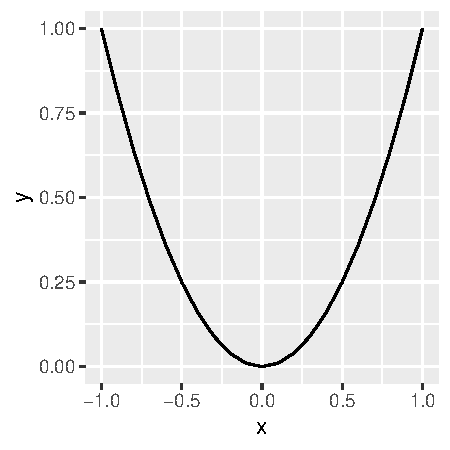
\includegraphics{bookdown-demo_files/figure-latex/unnamed-chunk-10-1.pdf}

\begin{Shaded}
\begin{Highlighting}[]
\NormalTok{q }\OtherTok{\textless{}{-}} \FunctionTok{ggplot}\NormalTok{(data, }\FunctionTok{aes}\NormalTok{(}\AttributeTok{x =}\NormalTok{ x, }\AttributeTok{y =}\NormalTok{ y1)) }\SpecialCharTok{+}
  \FunctionTok{geom\_line}\NormalTok{(}\AttributeTok{colour =} \StringTok{"red"}\NormalTok{)}
\FunctionTok{print}\NormalTok{(q)}
\end{Highlighting}
\end{Shaded}

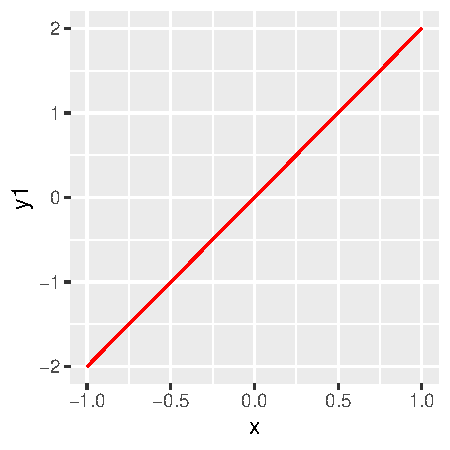
\includegraphics{bookdown-demo_files/figure-latex/unnamed-chunk-10-2.pdf}

\begin{Shaded}
\begin{Highlighting}[]
\NormalTok{r }\OtherTok{\textless{}{-}} \FunctionTok{ggplot}\NormalTok{(data, }\FunctionTok{aes}\NormalTok{(}\AttributeTok{x =}\NormalTok{ x, }\AttributeTok{y =}\NormalTok{ y2)) }\SpecialCharTok{+}
  \FunctionTok{geom\_line}\NormalTok{(}\AttributeTok{colour =} \StringTok{"blue"}\NormalTok{)}
\FunctionTok{print}\NormalTok{(r)}
\end{Highlighting}
\end{Shaded}

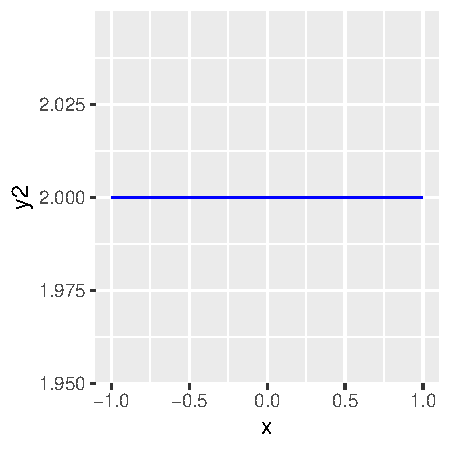
\includegraphics{bookdown-demo_files/figure-latex/unnamed-chunk-10-3.pdf}

\hypertarget{partial-derivatives}{%
\section{Partial Derivatives}\label{partial-derivatives}}

If the expression is having more than one independent variable, we can calculate differentiation with respect to each of them.

\begin{Shaded}
\begin{Highlighting}[]
\NormalTok{f }\OtherTok{\textless{}{-}} \FunctionTok{expression}\NormalTok{(x}\SpecialCharTok{\^{}}\DecValTok{2} \SpecialCharTok{+}\NormalTok{ y}\SpecialCharTok{\^{}}\DecValTok{2}\NormalTok{)}

\NormalTok{x }\OtherTok{\textless{}{-}}\NormalTok{ y }\OtherTok{\textless{}{-}} \FunctionTok{seq}\NormalTok{(}\SpecialCharTok{{-}}\DecValTok{3}\NormalTok{, }\DecValTok{3}\NormalTok{, }\AttributeTok{length =} \DecValTok{20}\NormalTok{)}
\NormalTok{surface }\OtherTok{\textless{}{-}} \ControlFlowTok{function}\NormalTok{(x, y) \{}
  \FunctionTok{eval}\NormalTok{(f)}
\NormalTok{\}}
\NormalTok{z }\OtherTok{\textless{}{-}} \FunctionTok{outer}\NormalTok{(x, y, surface)}
\FunctionTok{persp}\NormalTok{(x, y, z)}
\end{Highlighting}
\end{Shaded}

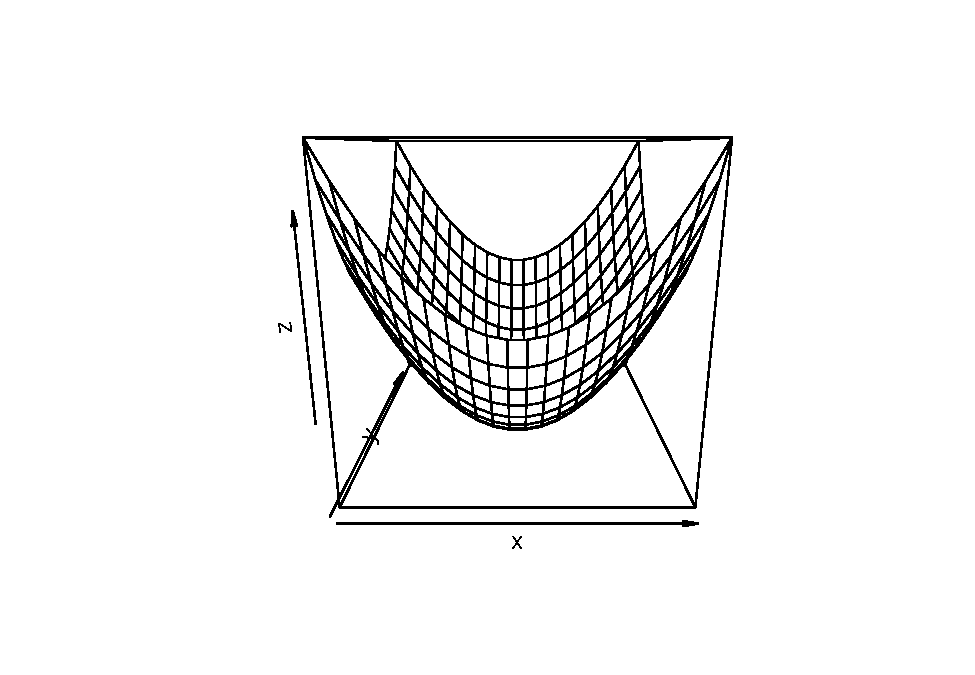
\includegraphics{bookdown-demo_files/figure-latex/unnamed-chunk-11-1.pdf}

Differentiate with respect to \texttt{x}

\begin{Shaded}
\begin{Highlighting}[]
\FunctionTok{D}\NormalTok{(f, }\StringTok{"x"}\NormalTok{)}
\end{Highlighting}
\end{Shaded}

\begin{verbatim}
## 2 * x
\end{verbatim}

Differentiate with respect to \texttt{y}

\begin{Shaded}
\begin{Highlighting}[]
\FunctionTok{D}\NormalTok{(f, }\StringTok{"y"}\NormalTok{)}
\end{Highlighting}
\end{Shaded}

\begin{verbatim}
## 2 * y
\end{verbatim}

\hypertarget{statistical-distributions}{%
\chapter{Statistical Distributions}\label{statistical-distributions}}

\begin{itemize}
\item
  Density, cumulative distribution function, quantile function and random variate generation for many standard probability distributions are available in the stats package.

  \begin{itemize}
  \tightlist
  \item
    dxxx : functions for the density/mass function,
  \item
    pxxx : cumulative distribution function
  \item
    qxxx : quantile function
  \item
    rxxx : random variable generation.
  \end{itemize}
\end{itemize}

\hypertarget{pxxx}{%
\section{pxxx}\label{pxxx}}

\textbf{Cumulative distribution function (lower tail probability)}

\emph{Example : Standard normal distribution}

\begin{itemize}
\item
  \texttt{pnorm(value-of-x-axis)} or \texttt{pnorm(quantile)}
\item
  \texttt{pnorm(0)\ =\ 0.5} (the area under the standard normal curve to the left of zero).
\end{itemize}

\begin{figure}

{\centering 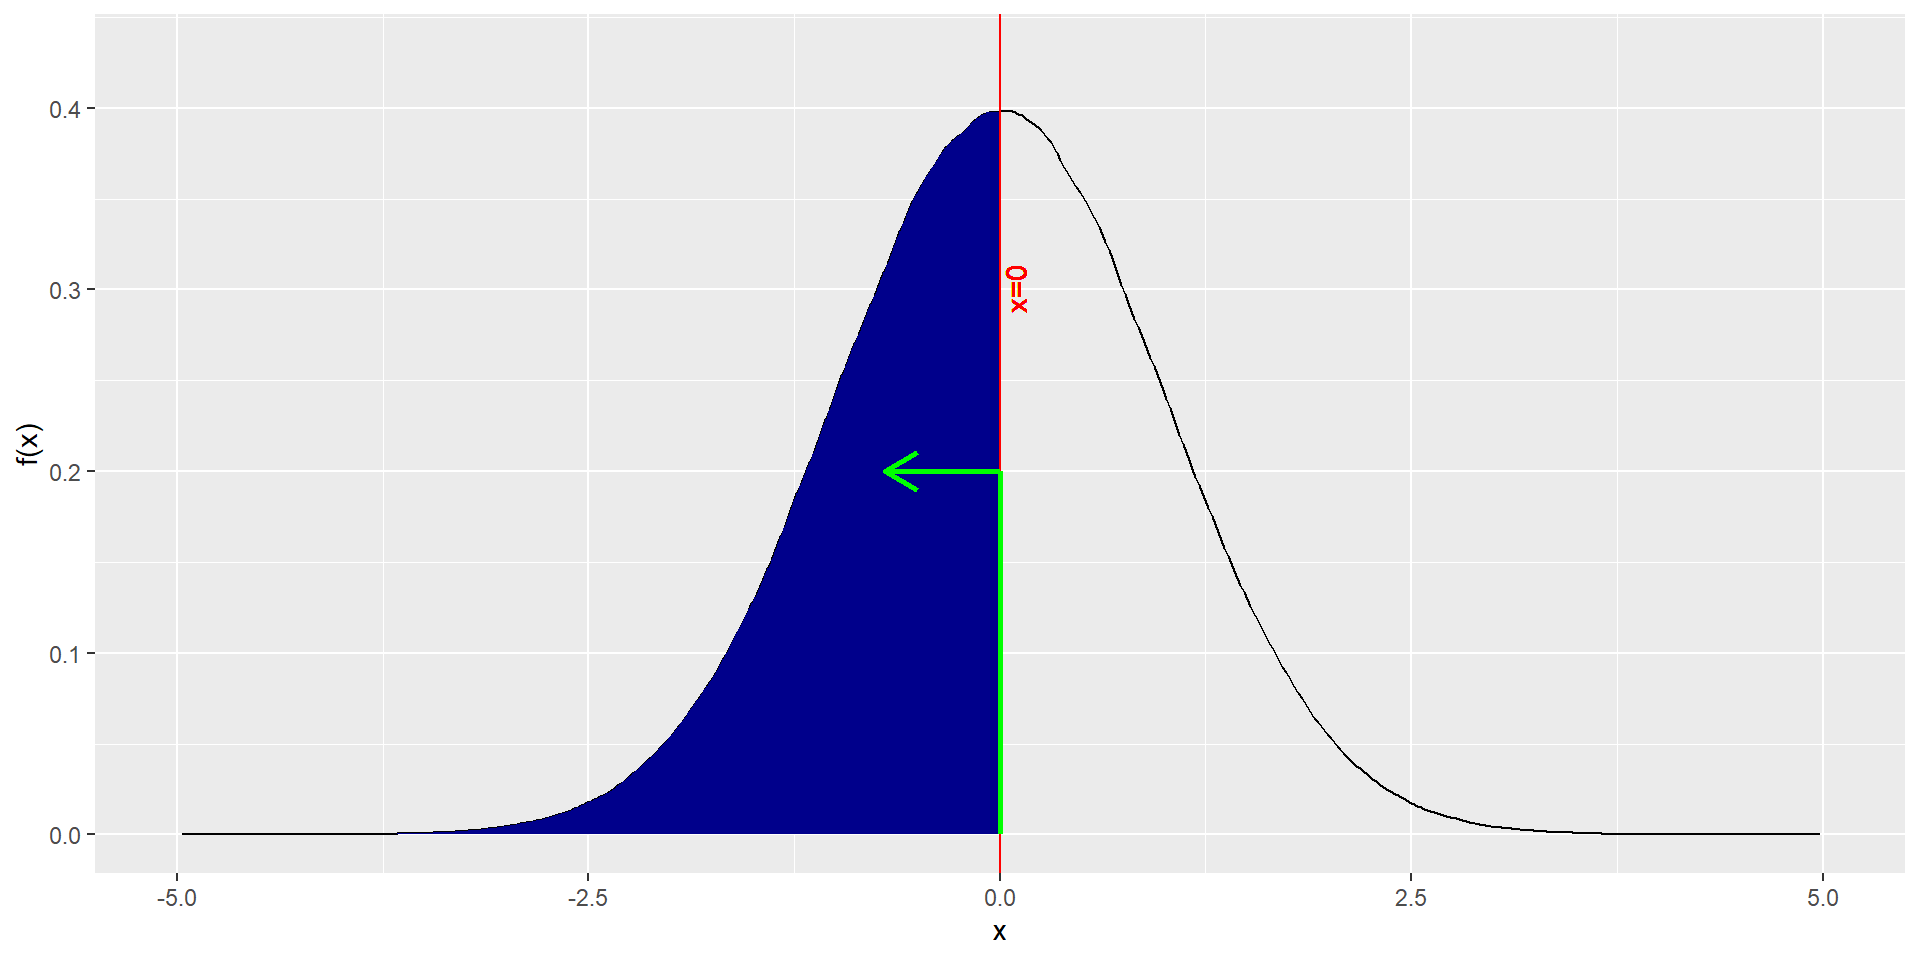
\includegraphics{figure/norm1-1} 

}

\caption{Standard normal distribution}\label{fig:norm1}
\end{figure}

\begin{itemize}
\tightlist
\item
  \texttt{pnorm(1.281552)\ =\ 0.9000} (the area under the standard normal curve to the left of 1.281).
\end{itemize}

\begin{figure}

{\centering 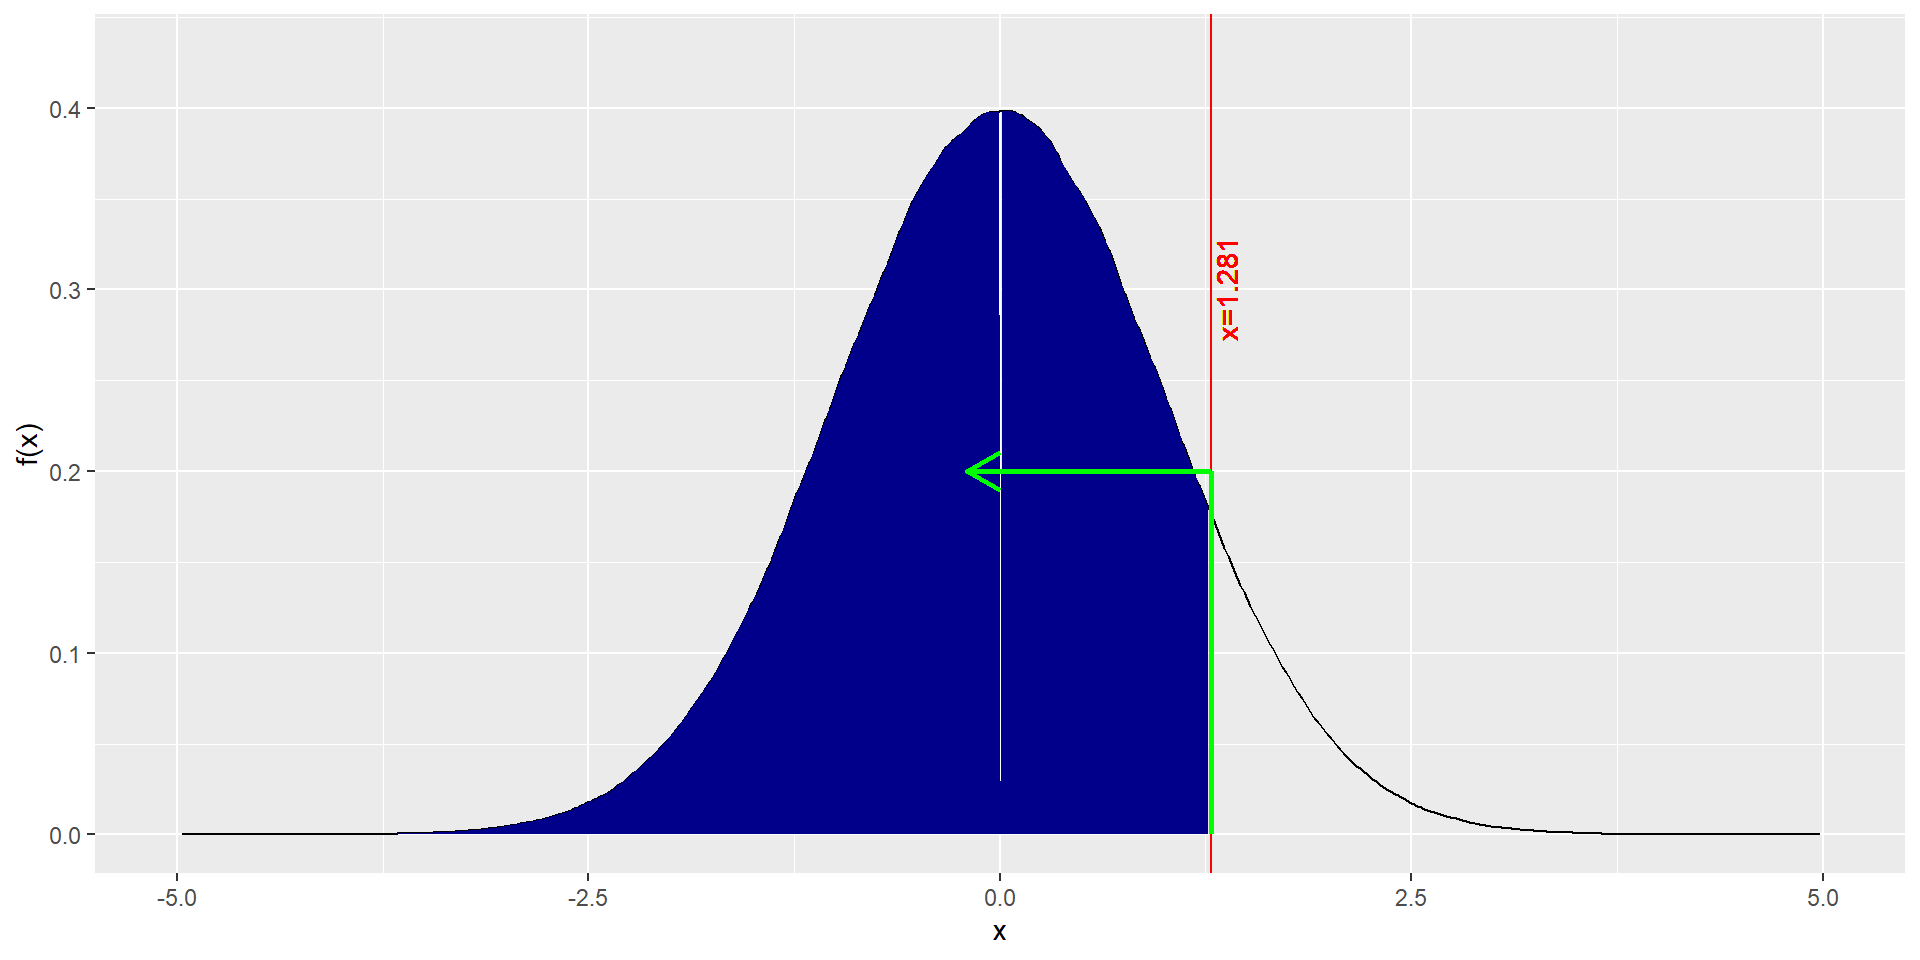
\includegraphics{figure/norm2-1} 

}

\caption{Standard normal distribution}\label{fig:norm2}
\end{figure}

\begin{itemize}
\item
  The \texttt{pnorm} function also takes the argument \texttt{lower.tail}. If \texttt{lower.tail} is set equal to \texttt{FALSE} then \texttt{pnorm} returns the upper tail probability (\emph{the integral from \(q\) to \(\infty\) of the pdf}) of the normal distribution.
\item
  Note that
\end{itemize}

\begin{Shaded}
\begin{Highlighting}[]
\FunctionTok{pnorm}\NormalTok{(}\FloatTok{1.281552}\NormalTok{)}
\end{Highlighting}
\end{Shaded}

\begin{verbatim}
## [1] 0.9000001
\end{verbatim}

\begin{Shaded}
\begin{Highlighting}[]
\FunctionTok{pnorm}\NormalTok{(}\FloatTok{1.281552}\NormalTok{, }\AttributeTok{lower.tail =} \ConstantTok{TRUE}\NormalTok{)}
\end{Highlighting}
\end{Shaded}

\begin{verbatim}
## [1] 0.9000001
\end{verbatim}

\begin{Shaded}
\begin{Highlighting}[]
\FunctionTok{pnorm}\NormalTok{(}\FloatTok{1.281552}\NormalTok{, }\AttributeTok{lower.tail =} \ConstantTok{FALSE}\NormalTok{) }
\end{Highlighting}
\end{Shaded}

\begin{verbatim}
## [1] 0.09999992
\end{verbatim}

\begin{Shaded}
\begin{Highlighting}[]
\DecValTok{1}\SpecialCharTok{{-}}\FunctionTok{pnorm}\NormalTok{(}\FloatTok{1.281552}\NormalTok{, }\AttributeTok{lower.tail =} \ConstantTok{TRUE}\NormalTok{)}
\end{Highlighting}
\end{Shaded}

\begin{verbatim}
## [1] 0.09999992
\end{verbatim}

\hypertarget{qxxx}{%
\section{qxxx}\label{qxxx}}

\emph{Example : Standard normal distribution}

\textbf{The \texttt{qnorm} function is simply the inverse of the cdf, which you can also think of as the inverse of \texttt{pnorm}!}

\begin{itemize}
\item
  \texttt{qnorm(probability)}
\item
  \texttt{qnorm(0.5)\ =\ 0} (0 is the 50th percentile of the standard normal distribution)
\end{itemize}

\begin{figure}

{\centering 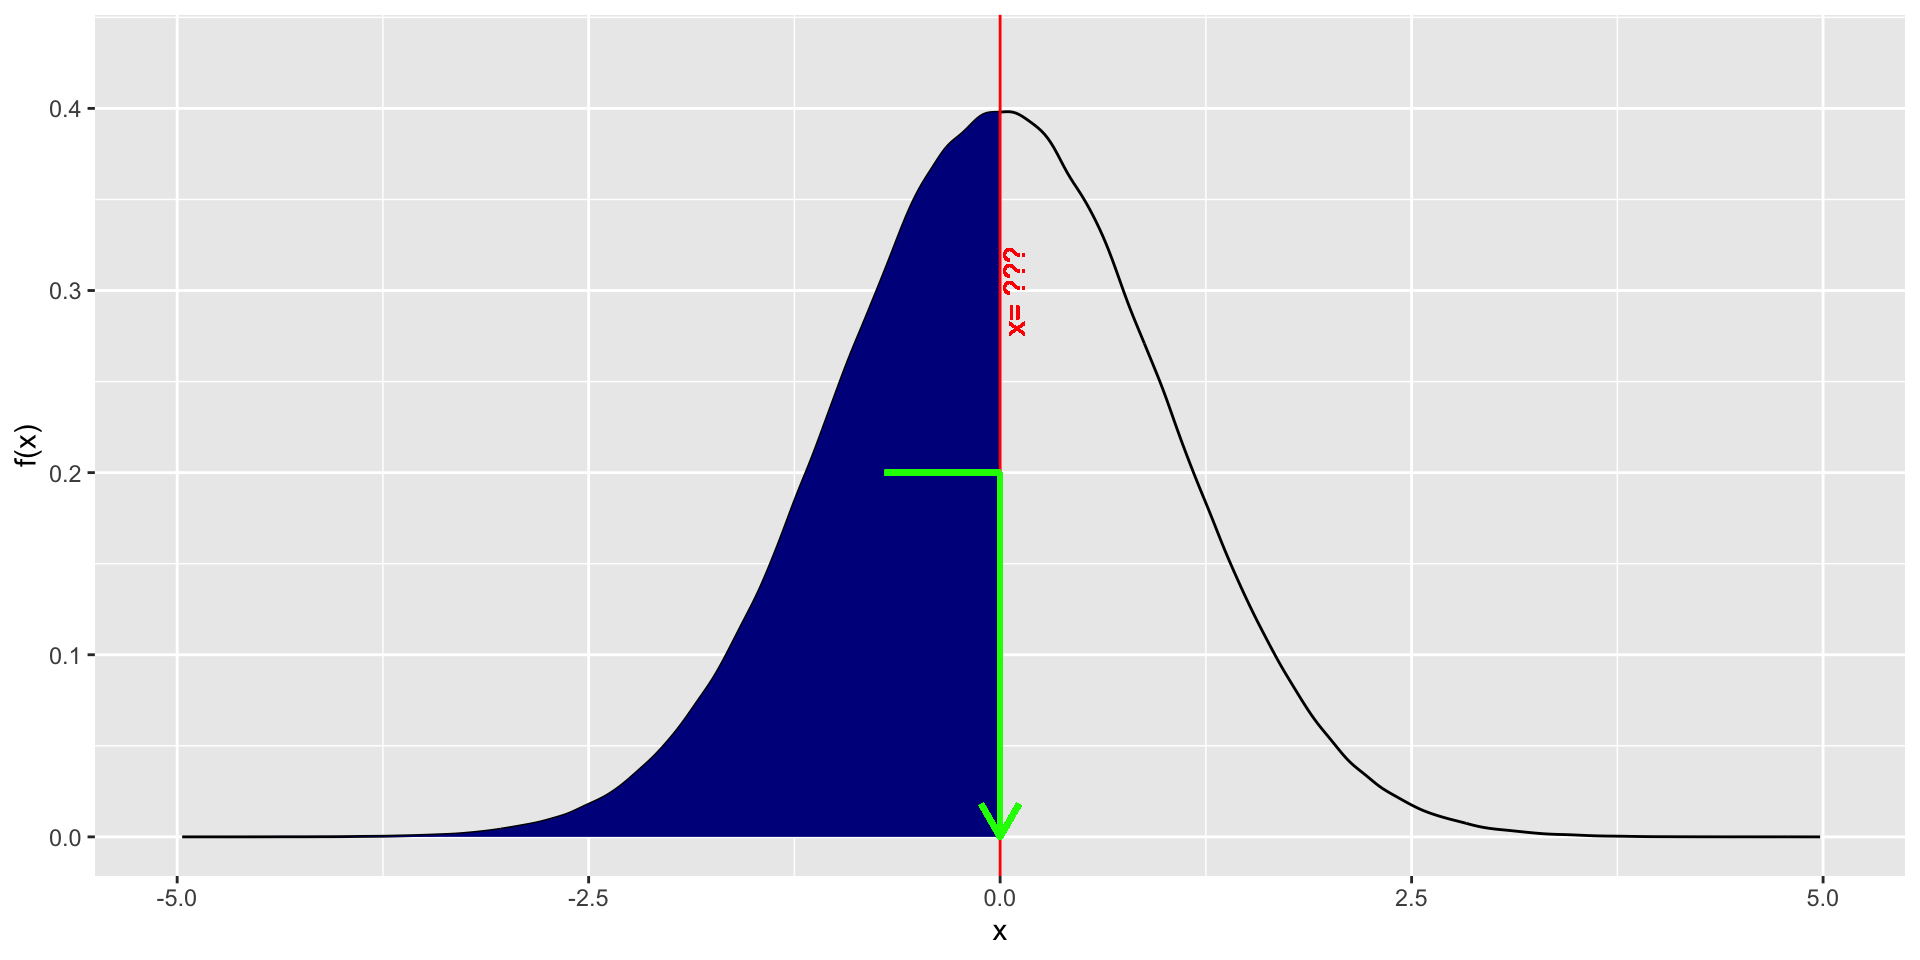
\includegraphics{figure/norm1b-1} 

}

\caption{Standard normal distribution}\label{fig:norm1b}
\end{figure}

\begin{Shaded}
\begin{Highlighting}[]
\FunctionTok{qnorm}\NormalTok{(}\FloatTok{0.5}\NormalTok{)}
\end{Highlighting}
\end{Shaded}

\begin{verbatim}
## [1] 0
\end{verbatim}

\begin{Shaded}
\begin{Highlighting}[]
\FunctionTok{qnorm}\NormalTok{(}\FloatTok{0.9}\NormalTok{)}
\end{Highlighting}
\end{Shaded}

\begin{verbatim}
## [1] 1.281552
\end{verbatim}

\begin{Shaded}
\begin{Highlighting}[]
\FunctionTok{qnorm}\NormalTok{(}\FloatTok{0.1}\NormalTok{, }\AttributeTok{lower.tail =} \ConstantTok{FALSE}\NormalTok{)}
\end{Highlighting}
\end{Shaded}

\begin{verbatim}
## [1] 1.281552
\end{verbatim}

\begin{Shaded}
\begin{Highlighting}[]
\FunctionTok{qnorm}\NormalTok{(}\FloatTok{0.9}\NormalTok{,  }\AttributeTok{lower.tail =} \ConstantTok{FALSE}\NormalTok{)}
\end{Highlighting}
\end{Shaded}

\begin{verbatim}
## [1] -1.281552
\end{verbatim}

\begin{figure}

{\centering 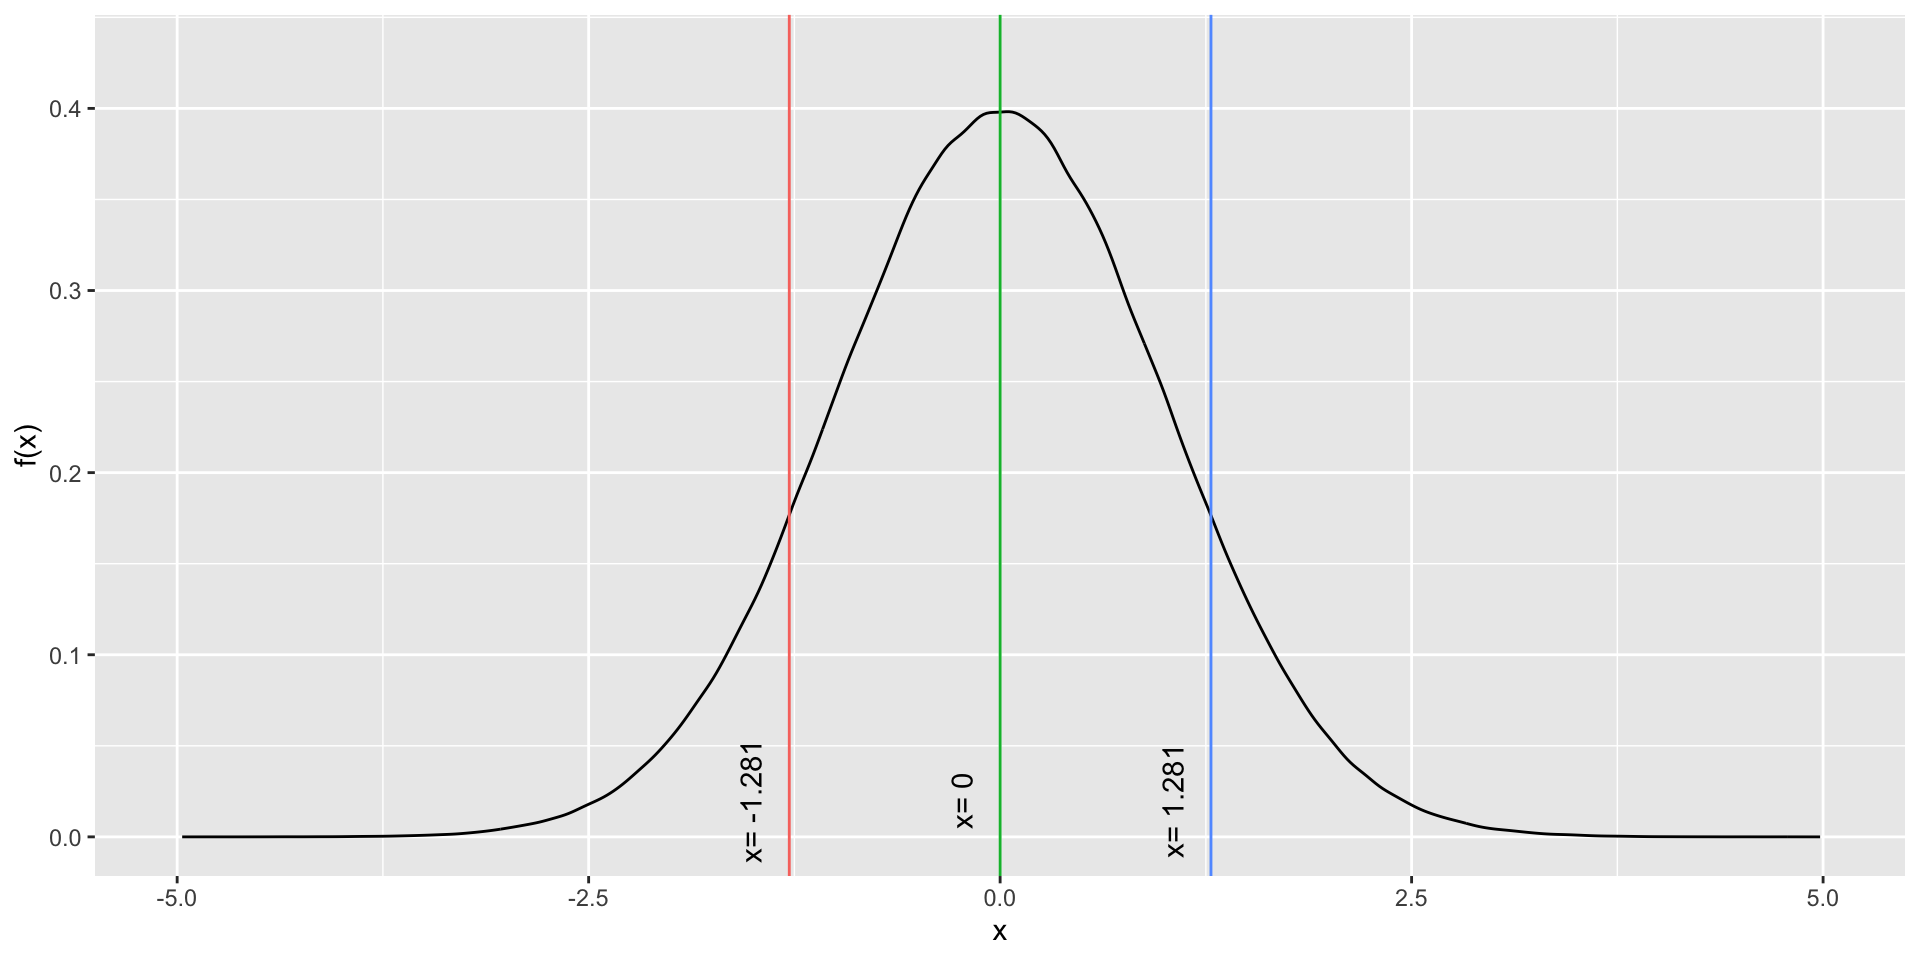
\includegraphics{figure/norm3-1} 

}

\caption{Standard normal distribution}\label{fig:norm3}
\end{figure}

\hypertarget{dxxx}{%
\section{dxxx}\label{dxxx}}

\emph{Example : Standard normal distribution}

\textbf{The function \texttt{dnorm} returns the value of the probability density function for the normal distribution given parameters for \(x\), \(\mu\), and \(\sigma\).}

\begin{itemize}
\tightlist
\item
  \texttt{dnorm(0)\ ==\ 1/sqrt(2*pi)}
\end{itemize}

If \(Z\sim N(0,1)\), then

\[\phi_Z(z) = \frac{1}{\sqrt{2 \pi}}e^{-\frac{1}{2}z^2};\;\; -\infty< z< \infty\]

\[\phi_Z(0) = \frac{1}{\sqrt{2 \pi}} =  0.3989423\]

\begin{Shaded}
\begin{Highlighting}[]
\FunctionTok{dnorm}\NormalTok{(}\DecValTok{0}\NormalTok{)}
\end{Highlighting}
\end{Shaded}

\begin{verbatim}
## [1] 0.3989423
\end{verbatim}

\begin{Shaded}
\begin{Highlighting}[]
\DecValTok{1}\SpecialCharTok{/}\FunctionTok{sqrt}\NormalTok{(}\DecValTok{2}\SpecialCharTok{*}\NormalTok{pi)}
\end{Highlighting}
\end{Shaded}

\begin{verbatim}
## [1] 0.3989423
\end{verbatim}

\begin{figure}

{\centering 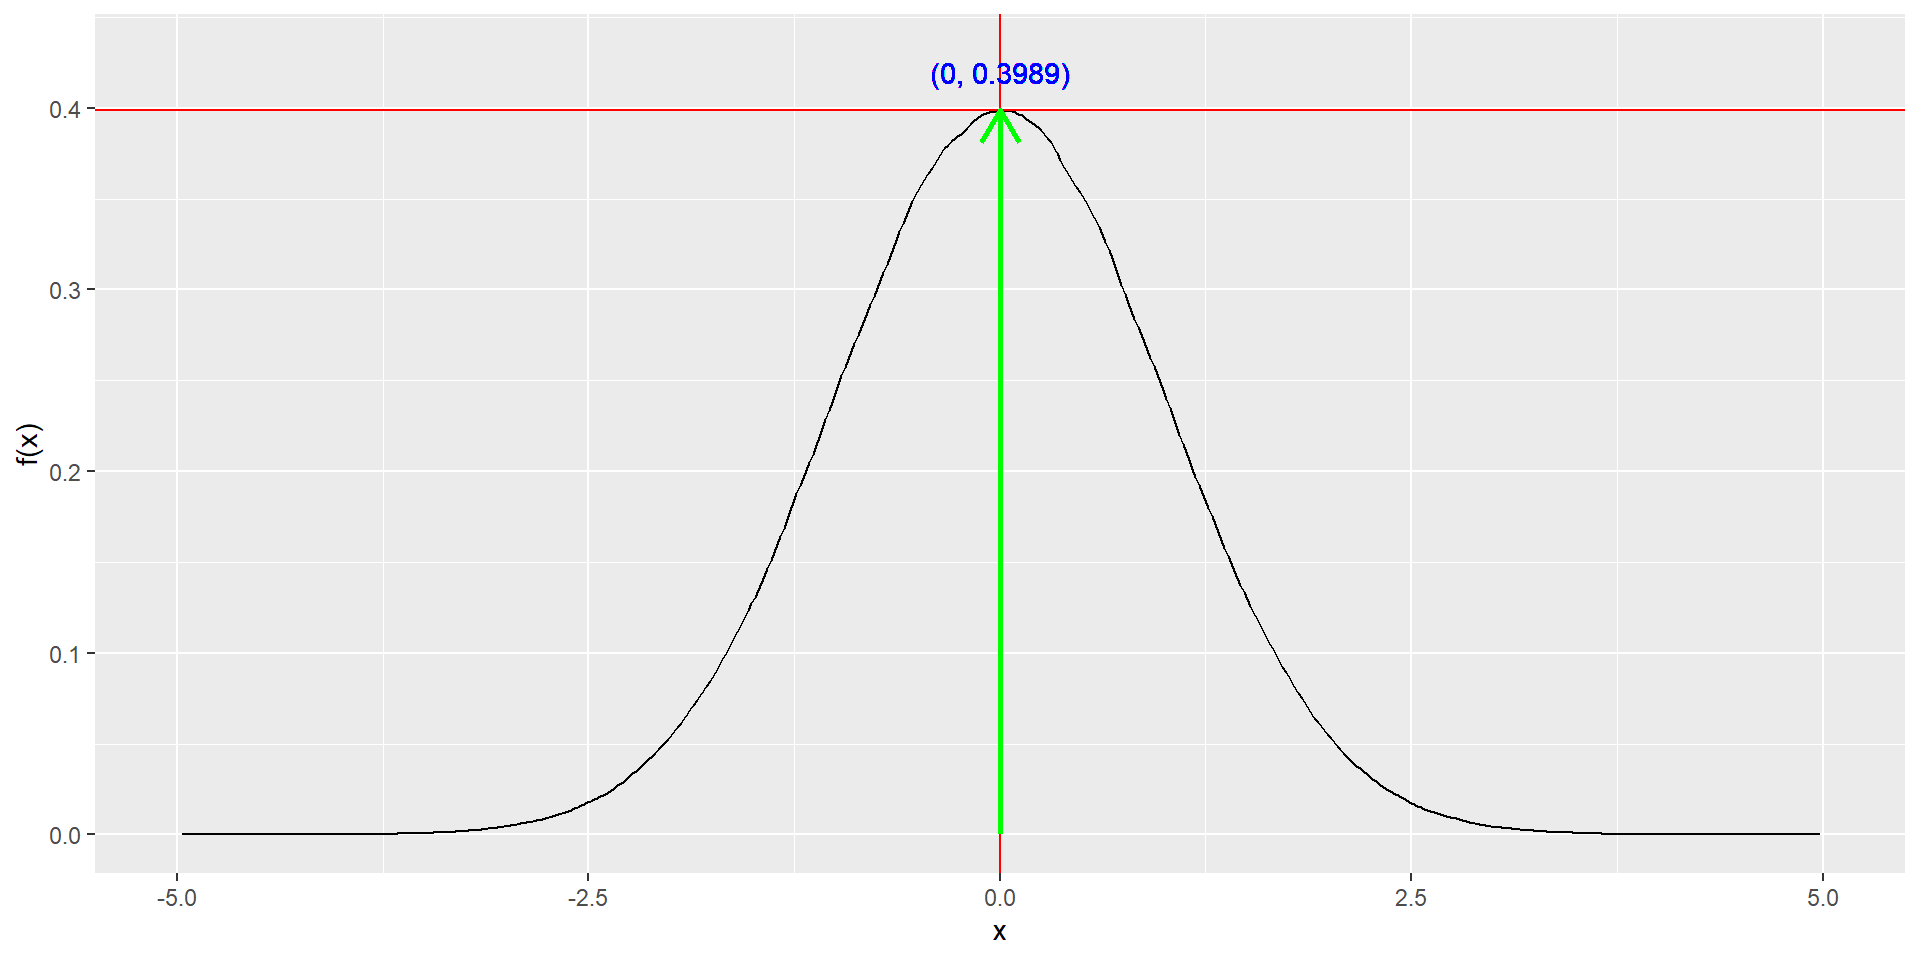
\includegraphics{figure/norm4-1} 

}

\caption{Standard normal distribution}\label{fig:norm4}
\end{figure}

\[\phi_Z(1) = \frac{1}{\sqrt{2 \pi}}e^{-\frac{1}{2}} =  0.3989423\]

\begin{Shaded}
\begin{Highlighting}[]
\FunctionTok{dnorm}\NormalTok{(}\DecValTok{1}\NormalTok{)}
\end{Highlighting}
\end{Shaded}

\begin{verbatim}
## [1] 0.2419707
\end{verbatim}

\begin{Shaded}
\begin{Highlighting}[]
\NormalTok{(}\DecValTok{1}\SpecialCharTok{/}\FunctionTok{sqrt}\NormalTok{(}\DecValTok{2}\SpecialCharTok{*}\NormalTok{pi)) }\SpecialCharTok{*} \FunctionTok{exp}\NormalTok{(}\SpecialCharTok{{-}}\DecValTok{1}\SpecialCharTok{/}\DecValTok{2}\NormalTok{)}
\end{Highlighting}
\end{Shaded}

\begin{verbatim}
## [1] 0.2419707
\end{verbatim}

\begin{figure}

{\centering 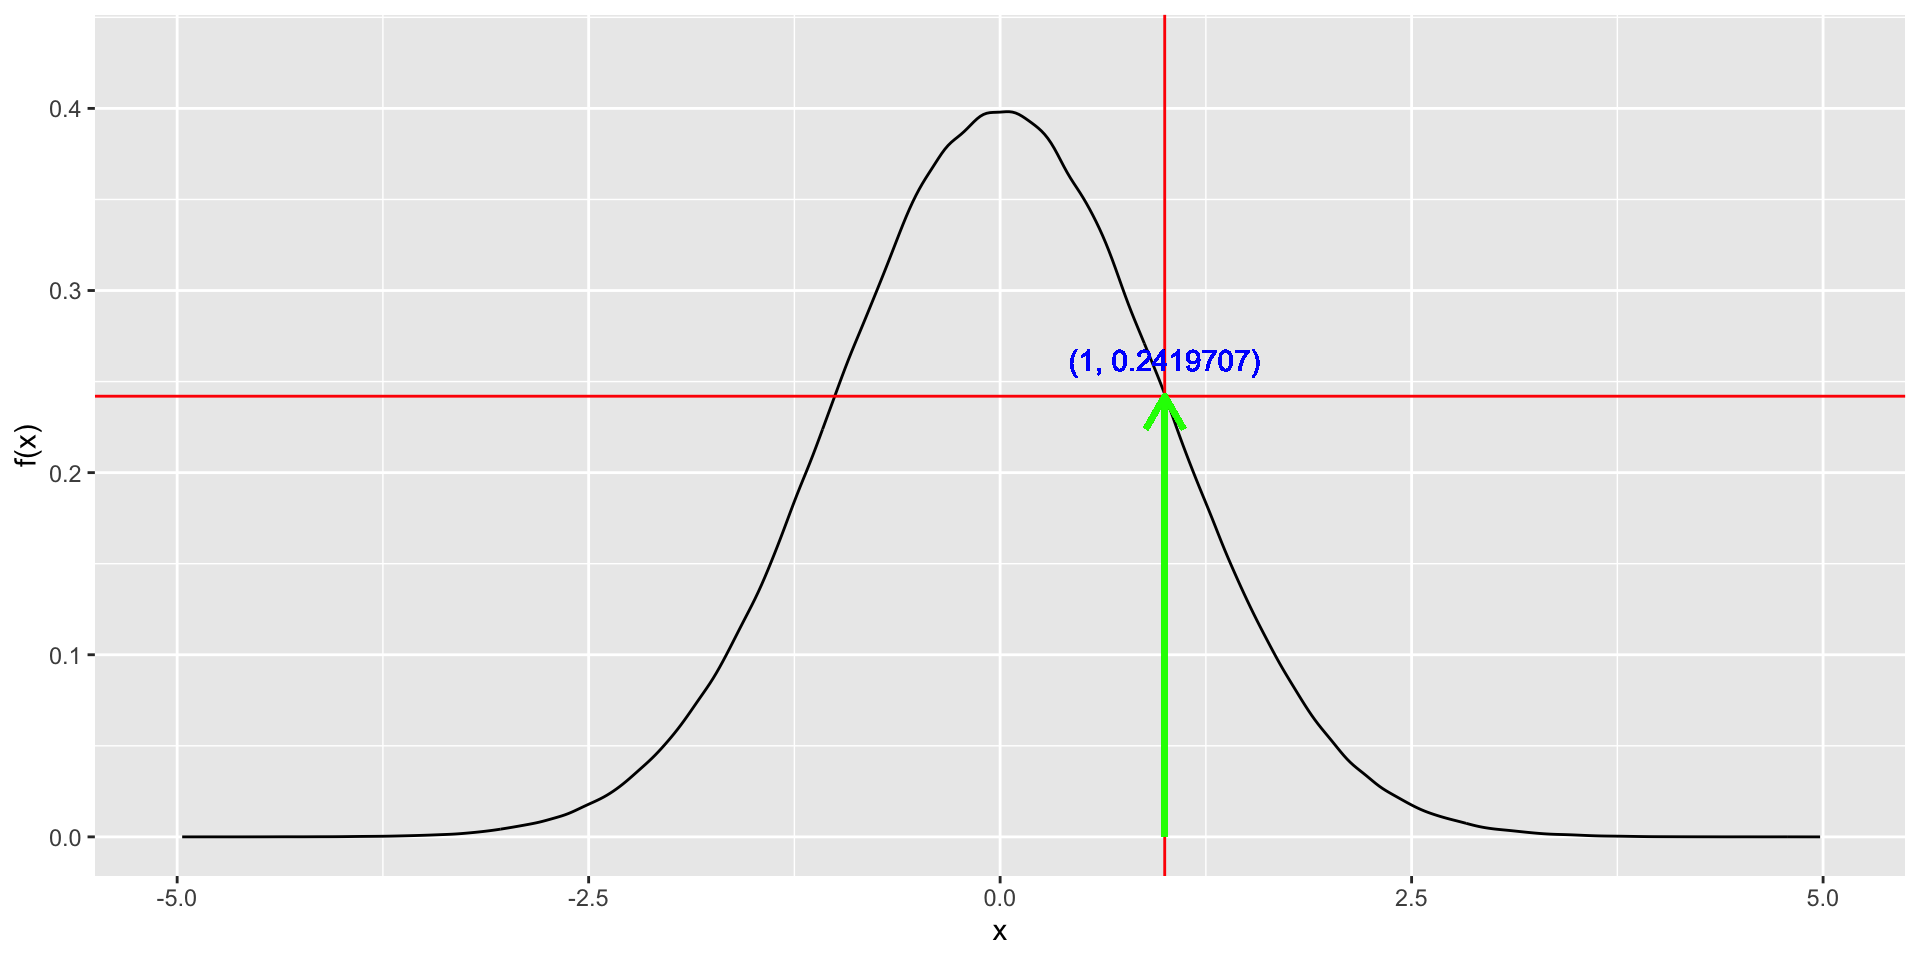
\includegraphics{figure/norm5-1} 

}

\caption{Standard normal distribution}\label{fig:norm5}
\end{figure}

\hypertarget{rxxx}{%
\section{rxxx}\label{rxxx}}

\emph{Example : Standard normal distribution}

\texttt{rnorm(100)} generates 100 random deviates from a standard normal distribution.

\begin{Shaded}
\begin{Highlighting}[]
\NormalTok{x }\OtherTok{\textless{}{-}} \FunctionTok{rnorm}\NormalTok{(}\DecValTok{10}\NormalTok{)}
\NormalTok{x}
\end{Highlighting}
\end{Shaded}

\begin{verbatim}
##  [1] -1.0080707  1.3549394 -0.4689749  1.4681936  0.4425564  0.1462031
##  [7]  0.1715031  0.5925072  2.7647493  0.6192188
\end{verbatim}

\begin{Shaded}
\begin{Highlighting}[]
\FunctionTok{hist}\NormalTok{(x)}
\end{Highlighting}
\end{Shaded}

\begin{center}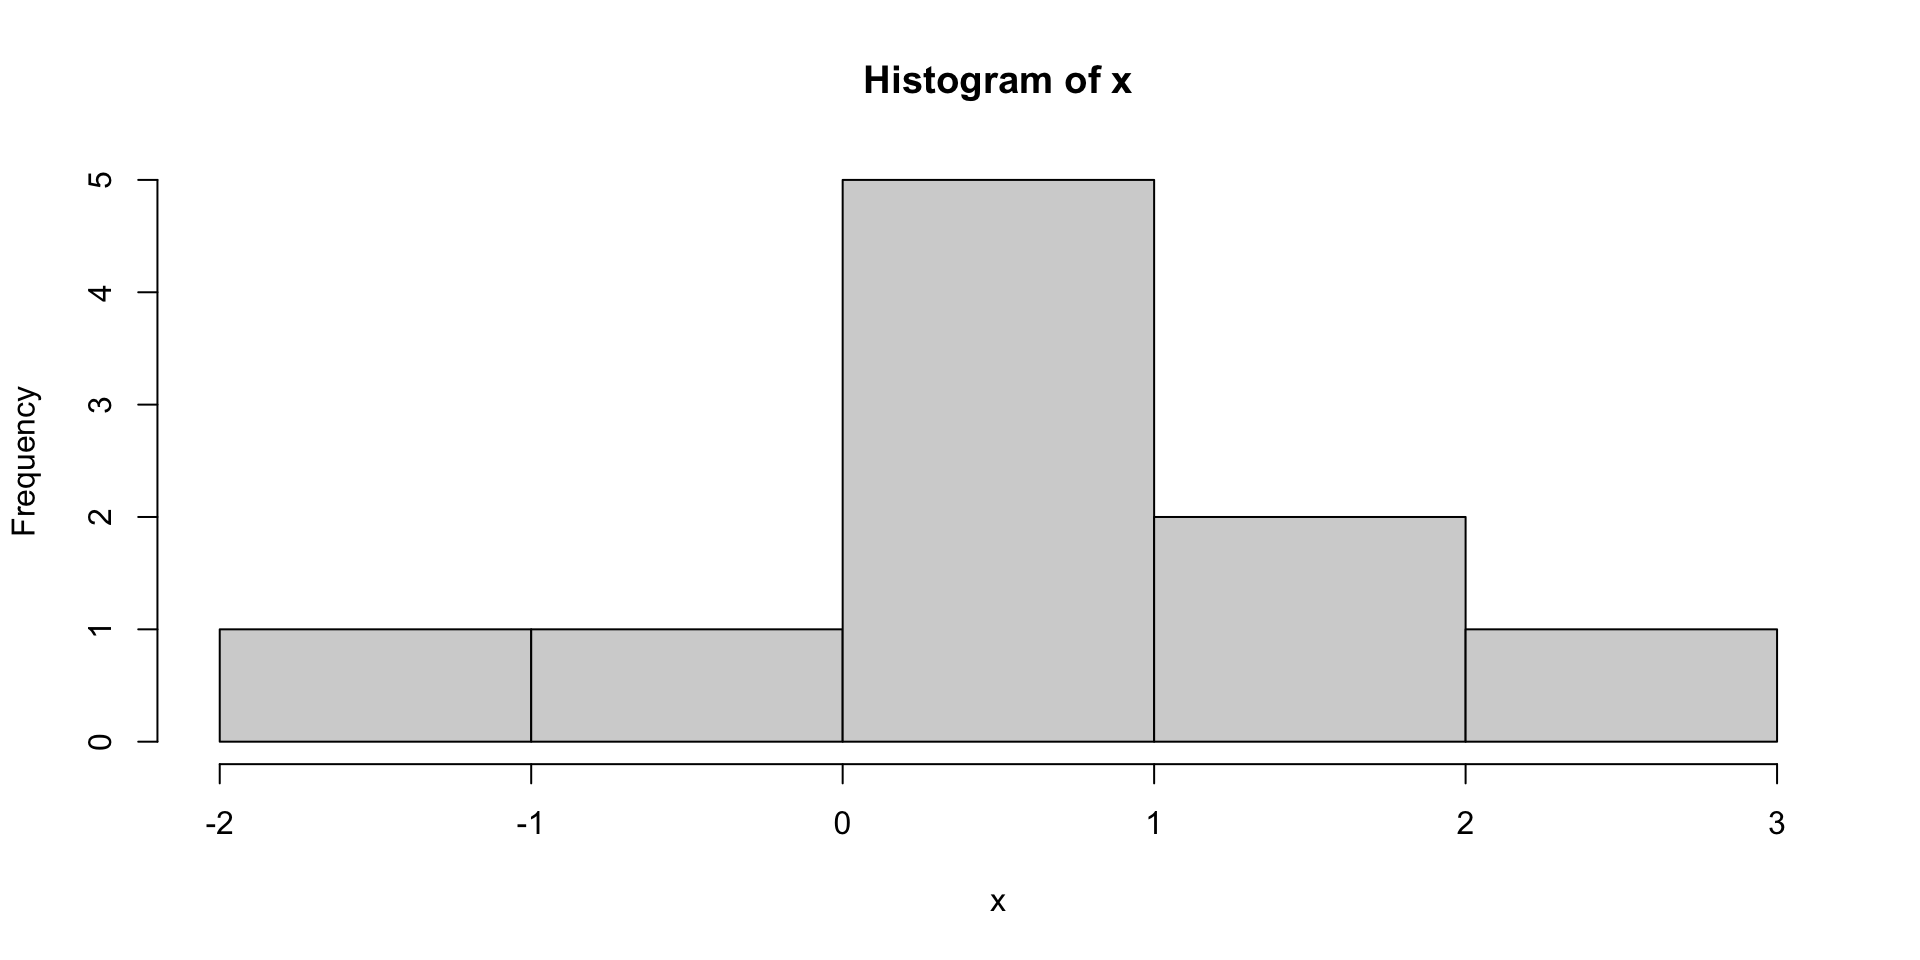
\includegraphics{figure/unnamed-chunk-18-1} \end{center}

\begin{Shaded}
\begin{Highlighting}[]
\NormalTok{y}\OtherTok{\textless{}{-}} \FunctionTok{rnorm}\NormalTok{(}\DecValTok{1000}\NormalTok{)}
\FunctionTok{hist}\NormalTok{(y)}
\end{Highlighting}
\end{Shaded}

\begin{center}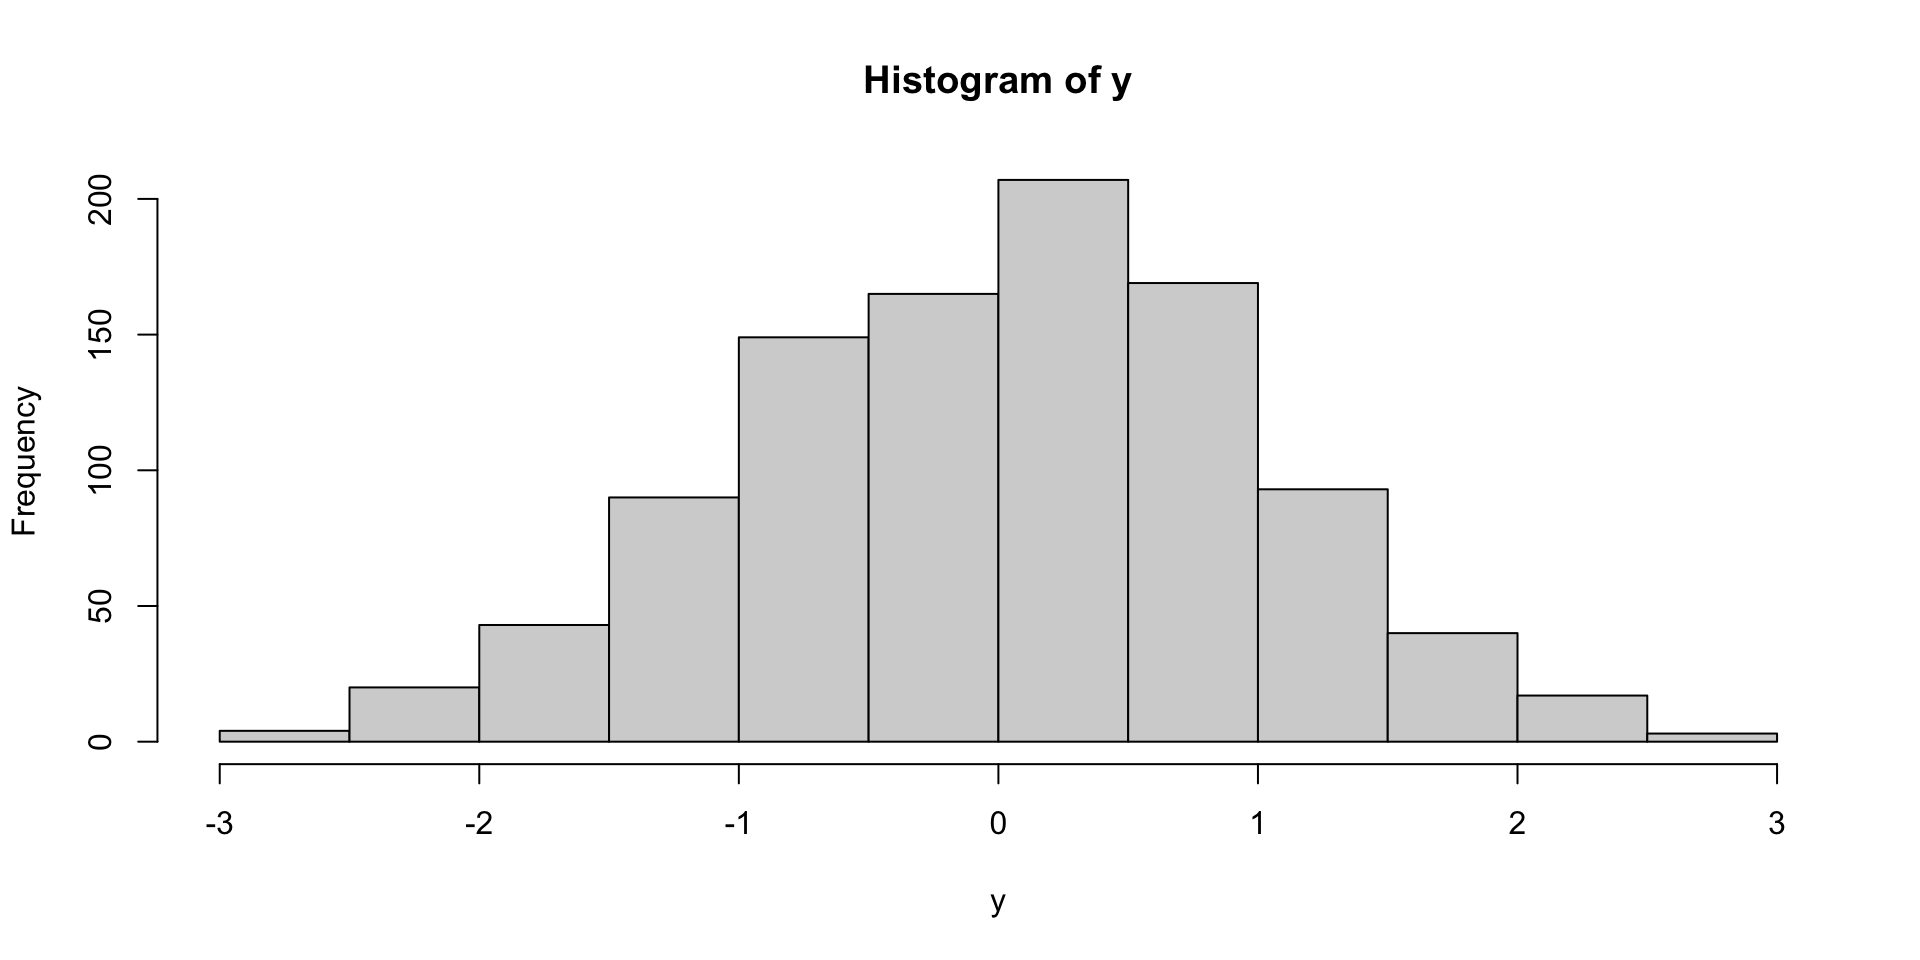
\includegraphics{figure/unnamed-chunk-19-1} \end{center}

\hypertarget{distributions-in-r}{%
\section{Distributions in R}\label{distributions-in-r}}

\begin{longtable}[]{@{}lll@{}}
\toprule()
Distribution & R name & Additional arguments \\
\midrule()
\endhead
beta & \texttt{beta} & \texttt{shape1,\ shape\ 2,\ ncp} \\
binomial & \texttt{binom} & \texttt{size,\ prob} \\
Cauchy & \texttt{cauchy} & \texttt{location,\ scale} \\
chi-squared & \texttt{chisq} & \texttt{df,\ ncp} \\
exponential & \texttt{exp} & \texttt{rate} \\
F & \texttt{f} & \texttt{df1,\ df2,\ ncp} \\
gamma & \texttt{gamma} & \texttt{shape,\ scale} \\
geometric & \texttt{geom} & \texttt{prob} \\
hypergeometric & \texttt{hyper} & \texttt{m,\ n,\ k} \\
log-normal & \texttt{lnorm} & \texttt{meanlog,\ sdlog} \\
logistic & \texttt{logis} & \texttt{location,\ scale} \\
negative binomial & \texttt{nbinom} & \texttt{size,\ prob} \\
normal & \texttt{norm} & \texttt{mean,\ sd} \\
Poisson & \texttt{pois} & \texttt{lambda} \\
signed rank & \texttt{signrank} & \texttt{n} \\
Student's t & \texttt{t} & \texttt{df,\ ncp} \\
uniform & \texttt{unif} & \texttt{min,\ max} \\
Weibull & \texttt{weibull} & \texttt{shape,\ scale} \\
Wilcoxon & \texttt{wilcox} & \texttt{m,\ n} \\
\bottomrule()
\end{longtable}

\hypertarget{exercise}{%
\section{Exercise}\label{exercise}}

\hypertarget{normal}{%
\subsection{Normal}\label{normal}}

\begin{figure}

{\centering 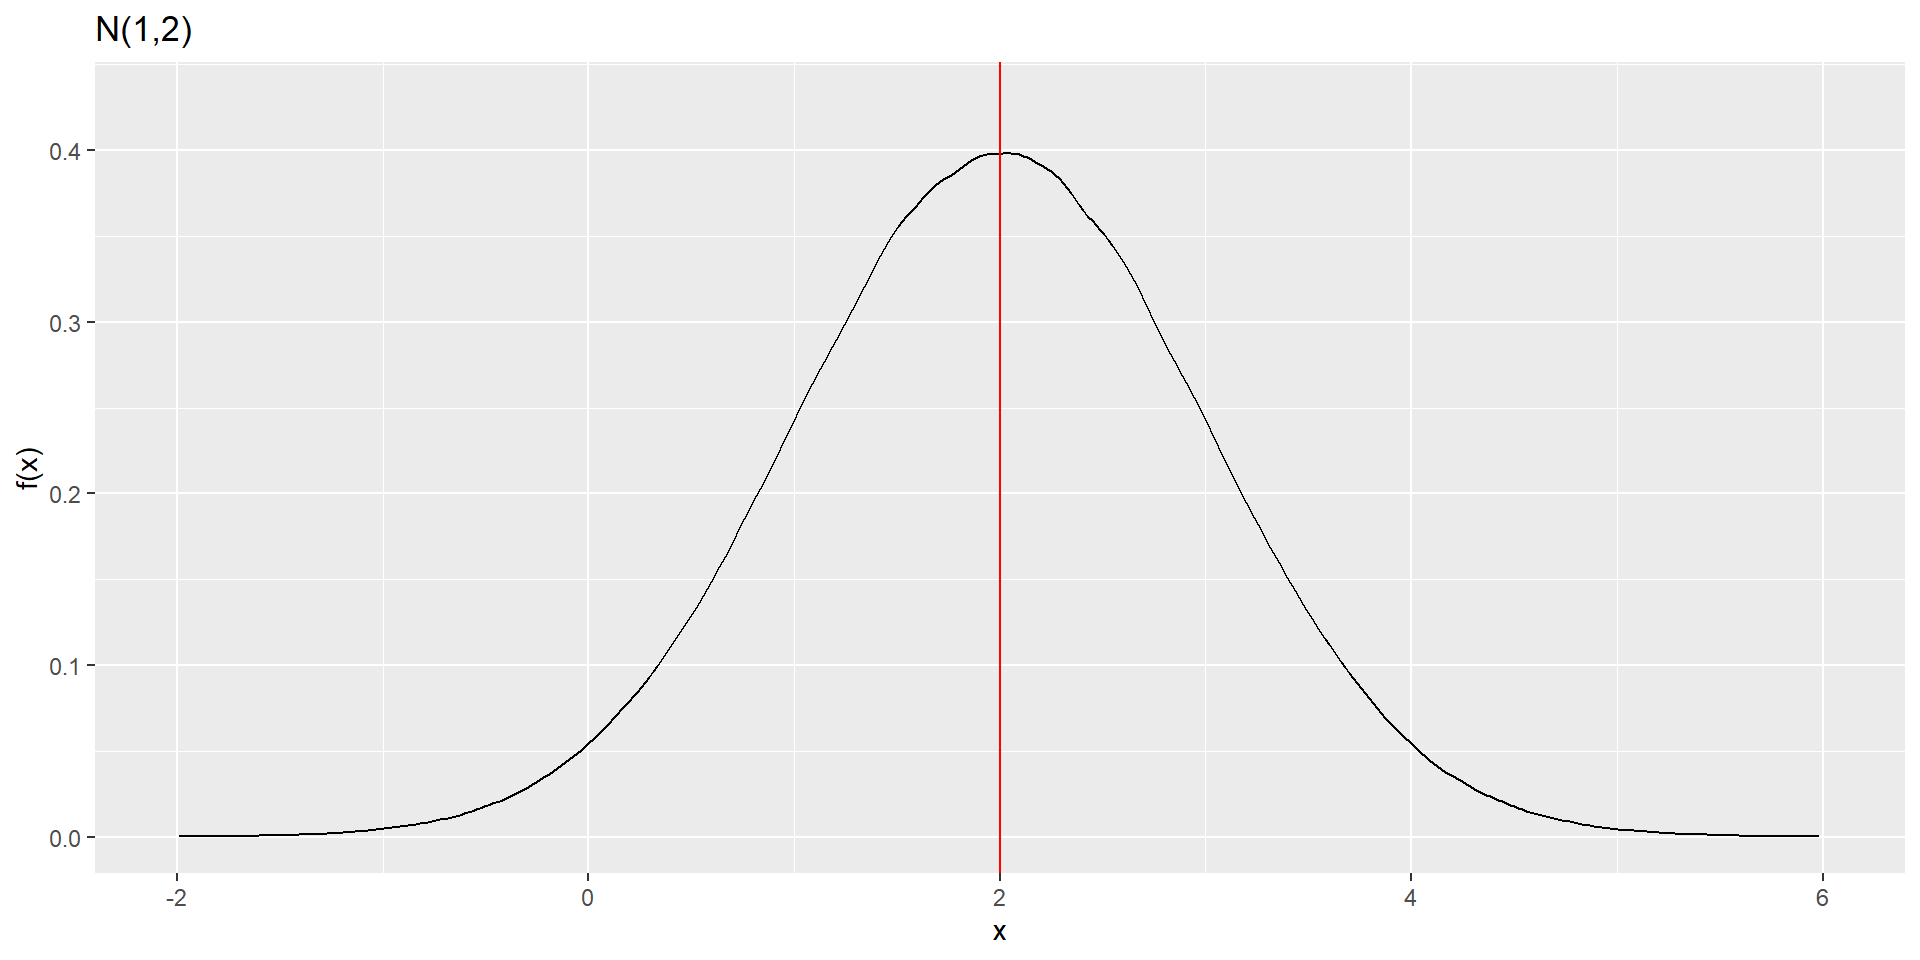
\includegraphics{figure/norm6-1} 

}

\caption{Standard normal distribution}\label{fig:norm6}
\end{figure}

\begin{Shaded}
\begin{Highlighting}[]
\CommentTok{\# ?dnorm {-} Help page}

\FunctionTok{dnorm}\NormalTok{(}\DecValTok{2}\NormalTok{, }\AttributeTok{mean =} \DecValTok{2}\NormalTok{, }\AttributeTok{sd =} \DecValTok{1}\NormalTok{, }\AttributeTok{log =} \ConstantTok{FALSE}\NormalTok{)}
\FunctionTok{pnorm}\NormalTok{(}\DecValTok{2}\NormalTok{, }\AttributeTok{mean =} \DecValTok{2}\NormalTok{, }\AttributeTok{sd =} \DecValTok{1}\NormalTok{, }\AttributeTok{lower.tail =} \ConstantTok{TRUE}\NormalTok{, }\AttributeTok{log.p =} \ConstantTok{FALSE}\NormalTok{)}
\FunctionTok{qnorm}\NormalTok{(}\FloatTok{0.5}\NormalTok{, }\AttributeTok{mean =} \DecValTok{2}\NormalTok{, }\AttributeTok{sd =} \DecValTok{1}\NormalTok{, }\AttributeTok{lower.tail =} \ConstantTok{TRUE}\NormalTok{, }\AttributeTok{log.p =} \ConstantTok{FALSE}\NormalTok{)}
\FunctionTok{rnorm}\NormalTok{(}\AttributeTok{n=}\DecValTok{10}\NormalTok{, }\AttributeTok{mean =} \DecValTok{2}\NormalTok{, }\AttributeTok{sd =} \DecValTok{1}\NormalTok{)}
\end{Highlighting}
\end{Shaded}

\begin{Shaded}
\begin{Highlighting}[]
\CommentTok{\# ?dnorm {-} Help page}

\FunctionTok{dnorm}\NormalTok{(}\DecValTok{2}\NormalTok{, }\AttributeTok{mean =} \DecValTok{2}\NormalTok{, }\AttributeTok{sd =} \DecValTok{1}\NormalTok{, }\AttributeTok{log =} \ConstantTok{FALSE}\NormalTok{)}
\end{Highlighting}
\end{Shaded}

\begin{verbatim}
## [1] 0.3989423
\end{verbatim}

\begin{Shaded}
\begin{Highlighting}[]
\FunctionTok{pnorm}\NormalTok{(}\DecValTok{2}\NormalTok{, }\AttributeTok{mean =} \DecValTok{2}\NormalTok{, }\AttributeTok{sd =} \DecValTok{1}\NormalTok{, }\AttributeTok{lower.tail =} \ConstantTok{TRUE}\NormalTok{, }\AttributeTok{log.p =} \ConstantTok{FALSE}\NormalTok{)}
\end{Highlighting}
\end{Shaded}

\begin{verbatim}
## [1] 0.5
\end{verbatim}

\begin{Shaded}
\begin{Highlighting}[]
\FunctionTok{qnorm}\NormalTok{(}\FloatTok{0.5}\NormalTok{, }\AttributeTok{mean =} \DecValTok{2}\NormalTok{, }\AttributeTok{sd =} \DecValTok{1}\NormalTok{, }\AttributeTok{lower.tail =} \ConstantTok{TRUE}\NormalTok{, }\AttributeTok{log.p =} \ConstantTok{FALSE}\NormalTok{)}
\end{Highlighting}
\end{Shaded}

\begin{verbatim}
## [1] 2
\end{verbatim}

\begin{Shaded}
\begin{Highlighting}[]
\FunctionTok{rnorm}\NormalTok{(}\AttributeTok{n=}\DecValTok{10}\NormalTok{, }\AttributeTok{mean =} \DecValTok{2}\NormalTok{, }\AttributeTok{sd =} \DecValTok{1}\NormalTok{)}
\end{Highlighting}
\end{Shaded}

\begin{verbatim}
##  [1] 0.9919293 3.3549394 1.5310251 3.4681936 2.4425564 2.1462031 2.1715031
##  [8] 2.5925072 4.7647493 2.6192188
\end{verbatim}

\hypertarget{gamma}{%
\subsection{Gamma}\label{gamma}}

\begin{figure}

{\centering 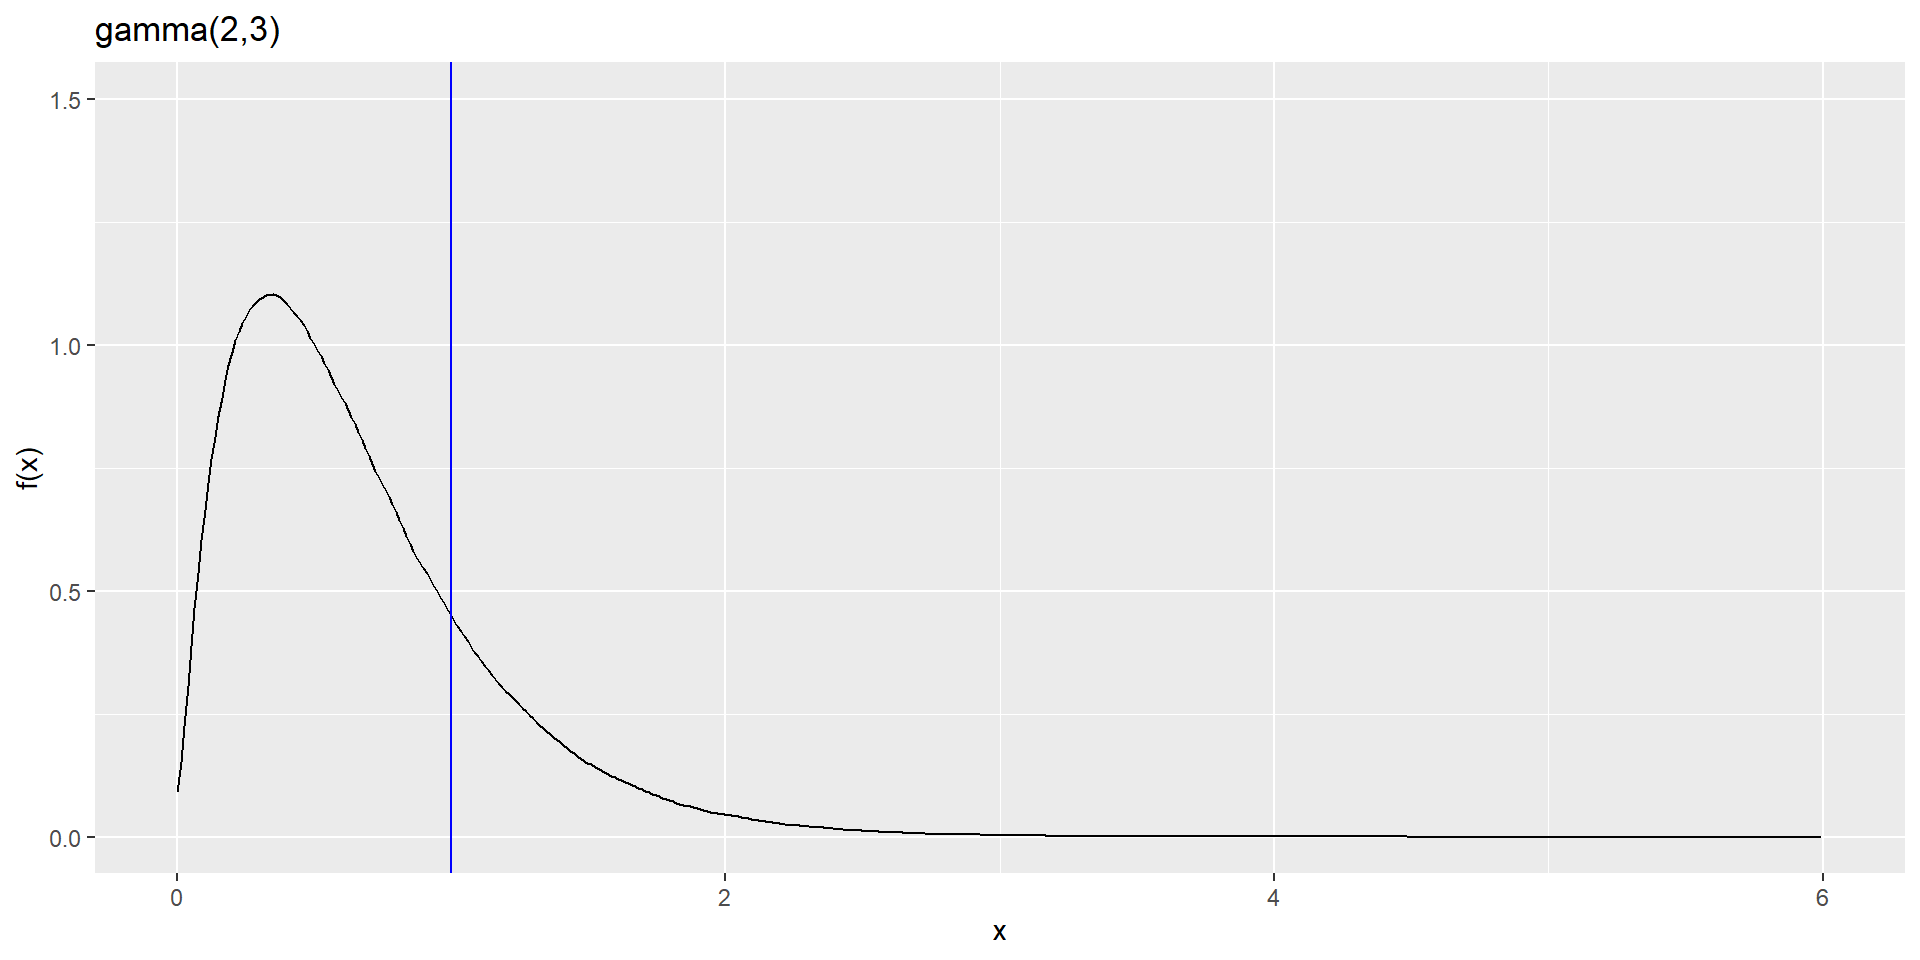
\includegraphics{figure/gamma-1} 

}

\caption{Standard normal distribution}\label{fig:gamma}
\end{figure}

\begin{Shaded}
\begin{Highlighting}[]
\FunctionTok{dgamma}\NormalTok{(}\DecValTok{1}\NormalTok{, }\AttributeTok{shape =}\DecValTok{2}\NormalTok{, }\AttributeTok{scale =} \DecValTok{1}\SpecialCharTok{/}\DecValTok{3}\NormalTok{, }\AttributeTok{log =} \ConstantTok{FALSE}\NormalTok{)}
\FunctionTok{pgamma}\NormalTok{(}\DecValTok{1}\NormalTok{, }\AttributeTok{shape =}\DecValTok{2}\NormalTok{, }\AttributeTok{scale =} \DecValTok{1}\SpecialCharTok{/}\DecValTok{3}\NormalTok{, }\AttributeTok{lower.tail =} \ConstantTok{TRUE}\NormalTok{,}
       \AttributeTok{log.p =} \ConstantTok{FALSE}\NormalTok{)}
\FunctionTok{qgamma}\NormalTok{(}\FloatTok{0.8}\NormalTok{, }\AttributeTok{shape =} \DecValTok{2}\NormalTok{,  }\AttributeTok{scale =} \DecValTok{1}\SpecialCharTok{/}\DecValTok{3}\NormalTok{, }\AttributeTok{lower.tail =} \ConstantTok{TRUE}\NormalTok{,}
       \AttributeTok{log.p =} \ConstantTok{FALSE}\NormalTok{)}
\FunctionTok{rgamma}\NormalTok{(}\DecValTok{10}\NormalTok{, }\AttributeTok{shape =}\DecValTok{2}\NormalTok{ , }\AttributeTok{scale =} \DecValTok{1}\SpecialCharTok{/}\DecValTok{3}\NormalTok{)}
\end{Highlighting}
\end{Shaded}

\begin{Shaded}
\begin{Highlighting}[]
\FunctionTok{dgamma}\NormalTok{(}\DecValTok{1}\NormalTok{, }\AttributeTok{shape =}\DecValTok{2}\NormalTok{, }\AttributeTok{scale =} \DecValTok{1}\SpecialCharTok{/}\DecValTok{3}\NormalTok{, }\AttributeTok{log =} \ConstantTok{FALSE}\NormalTok{)}
\end{Highlighting}
\end{Shaded}

\begin{verbatim}
## [1] 0.4480836
\end{verbatim}

\begin{Shaded}
\begin{Highlighting}[]
\FunctionTok{pgamma}\NormalTok{(}\DecValTok{1}\NormalTok{, }\AttributeTok{shape =}\DecValTok{2}\NormalTok{, }\AttributeTok{scale =} \DecValTok{1}\SpecialCharTok{/}\DecValTok{3}\NormalTok{, }\AttributeTok{lower.tail =} \ConstantTok{TRUE}\NormalTok{,}
       \AttributeTok{log.p =} \ConstantTok{FALSE}\NormalTok{)}
\end{Highlighting}
\end{Shaded}

\begin{verbatim}
## [1] 0.8008517
\end{verbatim}

\begin{Shaded}
\begin{Highlighting}[]
\FunctionTok{qgamma}\NormalTok{(}\FloatTok{0.8}\NormalTok{, }\AttributeTok{shape =} \DecValTok{2}\NormalTok{,  }\AttributeTok{scale =} \DecValTok{1}\SpecialCharTok{/}\DecValTok{3}\NormalTok{, }\AttributeTok{lower.tail =} \ConstantTok{TRUE}\NormalTok{,}
       \AttributeTok{log.p =} \ConstantTok{FALSE}\NormalTok{)}
\end{Highlighting}
\end{Shaded}

\begin{verbatim}
## [1] 0.9981028
\end{verbatim}

\begin{Shaded}
\begin{Highlighting}[]
\FunctionTok{rgamma}\NormalTok{(}\DecValTok{10}\NormalTok{, }\AttributeTok{shape =}\DecValTok{2}\NormalTok{ , }\AttributeTok{scale =} \DecValTok{1}\SpecialCharTok{/}\DecValTok{3}\NormalTok{)}
\end{Highlighting}
\end{Shaded}

\begin{verbatim}
##  [1] 0.3117027 0.5663228 1.8567817 0.1403567 0.7776307 0.8252981 1.4063366
##  [8] 0.7292312 0.9434481 0.9001169
\end{verbatim}

\newpage

\hypertarget{references}{%
\section{References}\label{references}}

Discrete
\url{http://www.r-tutor.com/elementary-statistics/probability-distributions}

\url{https://rstudio-pubs-static.s3.amazonaws.com/100906_8e3a32dd11c14b839468db756cee7400.html}

\hypertarget{linear-regression-in-r}{%
\chapter*{Linear Regression in R}\label{linear-regression-in-r}}
\addcontentsline{toc}{chapter}{Linear Regression in R}

\pagenumbering{arabic}

In many practical situations we want to identify various types of relationships between variables. \textbf{Regression analysis} is a statistical technique for investigating and \textbf{modeling the relationship between variables}.

\textbf{Linear regression} attempts to model the relationship between a scalar response (or dependent variable) and one or more explanatory variables (or independent variables) by fitting a \textbf{linear equation} to observed data. The case of one explanatory variable is called \textbf{simple linear regression.}

\hypertarget{loading-required-r-packages}{%
\section{Loading required R packages}\label{loading-required-r-packages}}

The following R packages are required for this chapter:

\begin{itemize}
\tightlist
\item
  \texttt{ggplot2} for data visualization
\item
  \texttt{datarium} data bank for statistical analysis and visualization
\item
  The \texttt{ggpairs()} function of the \texttt{GGally} package allows to build a great scatterplot matrix.
\end{itemize}

\begin{Shaded}
\begin{Highlighting}[]
\FunctionTok{library}\NormalTok{(ggplot2)}
\FunctionTok{library}\NormalTok{(datarium)}
\DocumentationTok{\#\# To learn more about the dataset}
\CommentTok{\# ?marketing}

\FunctionTok{library}\NormalTok{(GGally)}
\end{Highlighting}
\end{Shaded}

\begin{itemize}
\tightlist
\item
  We are going to use the marketing data set available in \texttt{datarium} package, which contains the impact of the amount of money spent on three advertising medias (youtube, Facebook and newspaper) on sales.
\end{itemize}

\hypertarget{load-data-set}{%
\section{Load Data set}\label{load-data-set}}

\begin{Shaded}
\begin{Highlighting}[]
\FunctionTok{data}\NormalTok{(marketing)}
\FunctionTok{head}\NormalTok{(marketing)}
\end{Highlighting}
\end{Shaded}

\begin{verbatim}
##   youtube facebook newspaper sales
## 1  276.12    45.36     83.04 26.52
## 2   53.40    47.16     54.12 12.48
## 3   20.64    55.08     83.16 11.16
## 4  181.80    49.56     70.20 22.20
## 5  216.96    12.96     70.08 15.48
## 6   10.44    58.68     90.00  8.64
\end{verbatim}

\begin{Shaded}
\begin{Highlighting}[]
\FunctionTok{summary}\NormalTok{(marketing)}
\end{Highlighting}
\end{Shaded}

\begin{verbatim}
##     youtube          facebook       newspaper          sales      
##  Min.   :  0.84   Min.   : 0.00   Min.   :  0.36   Min.   : 1.92  
##  1st Qu.: 89.25   1st Qu.:11.97   1st Qu.: 15.30   1st Qu.:12.45  
##  Median :179.70   Median :27.48   Median : 30.90   Median :15.48  
##  Mean   :176.45   Mean   :27.92   Mean   : 36.66   Mean   :16.83  
##  3rd Qu.:262.59   3rd Qu.:43.83   3rd Qu.: 54.12   3rd Qu.:20.88  
##  Max.   :355.68   Max.   :59.52   Max.   :136.80   Max.   :32.40
\end{verbatim}

\hypertarget{explore-data}{%
\section{Explore data}\label{explore-data}}

\hypertarget{scatterplot}{%
\subsection{Scatterplot}\label{scatterplot}}

\begin{itemize}
\tightlist
\item
  Usually, the first step in regression analysis is to construct a scatter plot (or scatter matrix).
\end{itemize}

\begin{Shaded}
\begin{Highlighting}[]
\FunctionTok{ggplot}\NormalTok{(}\AttributeTok{data =}\NormalTok{ marketing, }\FunctionTok{aes}\NormalTok{(}\AttributeTok{x =}\NormalTok{ facebook, }\AttributeTok{y =}\NormalTok{ sales)) }\SpecialCharTok{+}
  \FunctionTok{geom\_point}\NormalTok{() }\SpecialCharTok{+}
  \FunctionTok{theme}\NormalTok{(}\AttributeTok{aspect.ratio =} \DecValTok{1}\NormalTok{)}\SpecialCharTok{+}
  \FunctionTok{xlab}\NormalTok{(}\StringTok{"Sales"}\NormalTok{)}\SpecialCharTok{+}
  \FunctionTok{ylab}\NormalTok{(}\StringTok{"facebook"}\NormalTok{)}
\end{Highlighting}
\end{Shaded}

\begin{center}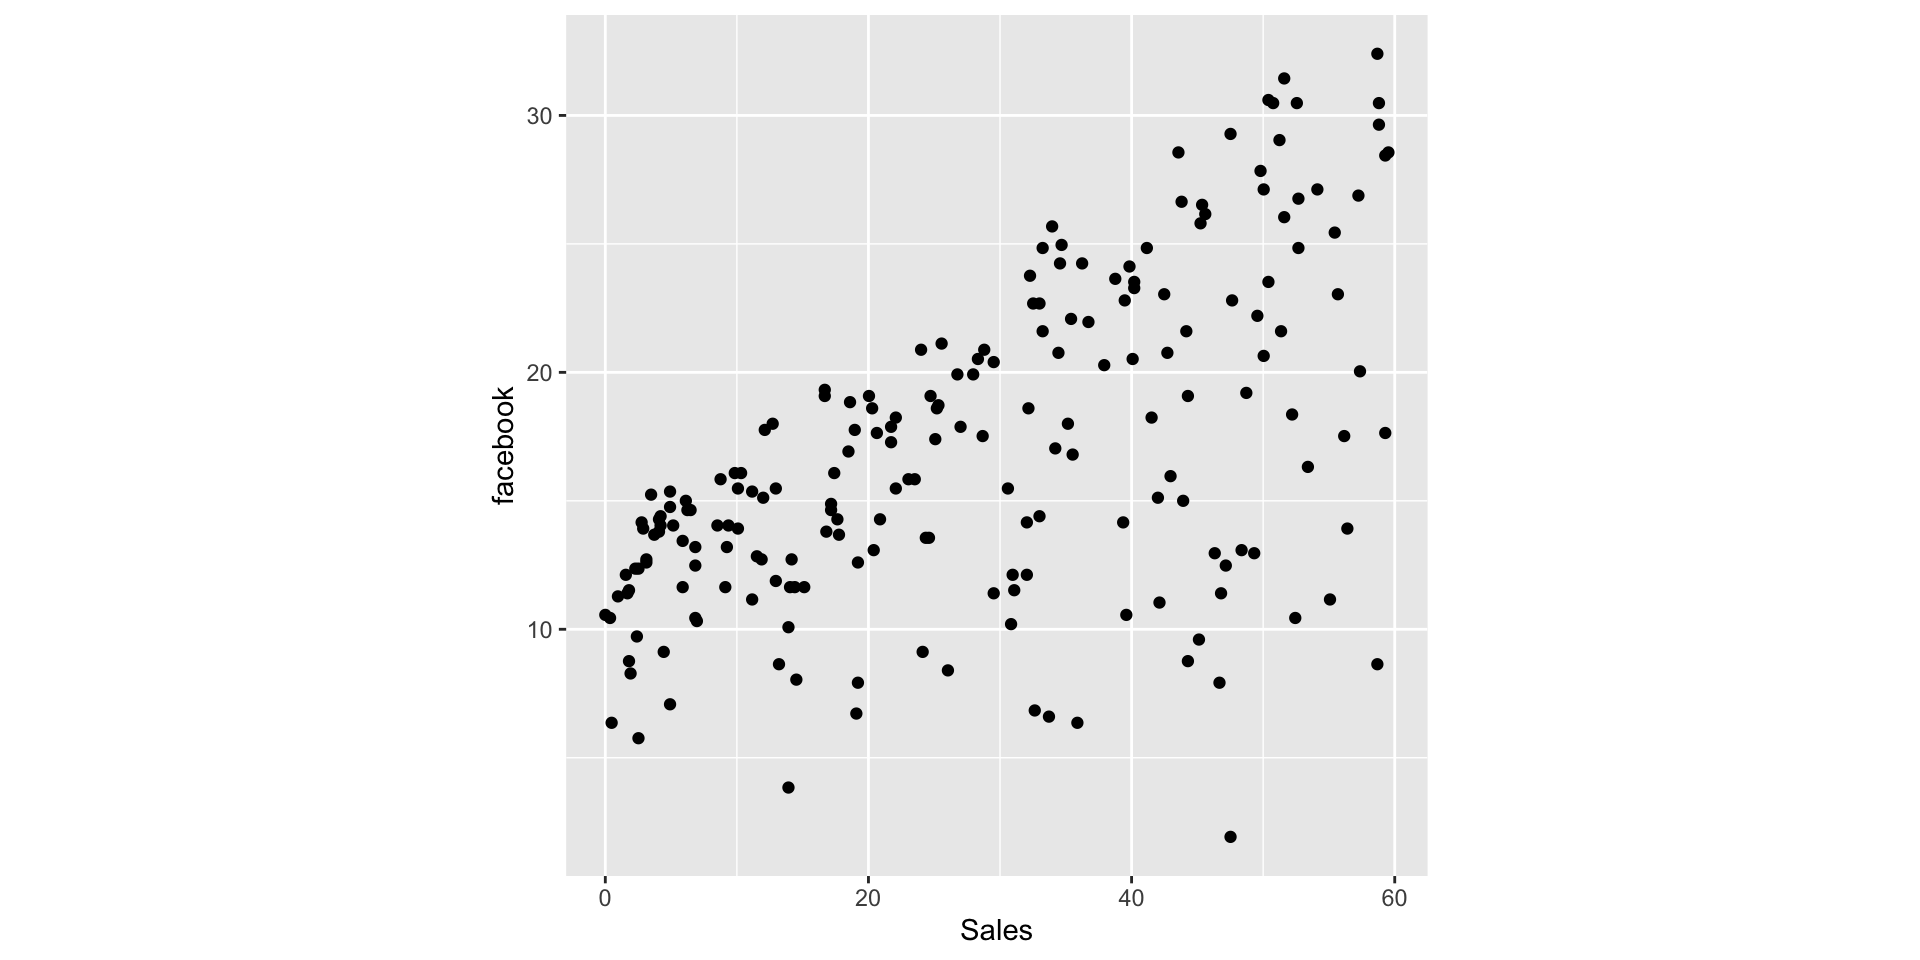
\includegraphics{figure/unnamed-chunk-26-1} \end{center}

\hypertarget{scatterplot-matrix}{%
\subsection{Scatterplot matrix}\label{scatterplot-matrix}}

\begin{itemize}
\tightlist
\item
  The \texttt{ggpairs()} function of the \texttt{GGally} package allows to build a great scatterplot matrix.
\item
  Scatterplots of each pair of numeric variable are drawn on the left part of the figure.
\item
  Pearson correlation is displayed on the right.
\item
  Variable distribution is available on the diagonal.
\end{itemize}

\begin{Shaded}
\begin{Highlighting}[]
\CommentTok{\# Check correlations (as scatterplots), distribution and print corrleation coefficient }

\FunctionTok{ggpairs}\NormalTok{(marketing, }\AttributeTok{title=}\StringTok{"correlogram with ggpairs()"}\NormalTok{) }\SpecialCharTok{+}
   \FunctionTok{theme}\NormalTok{(}\AttributeTok{aspect.ratio =} \DecValTok{1}\NormalTok{)}
\end{Highlighting}
\end{Shaded}

\begin{center}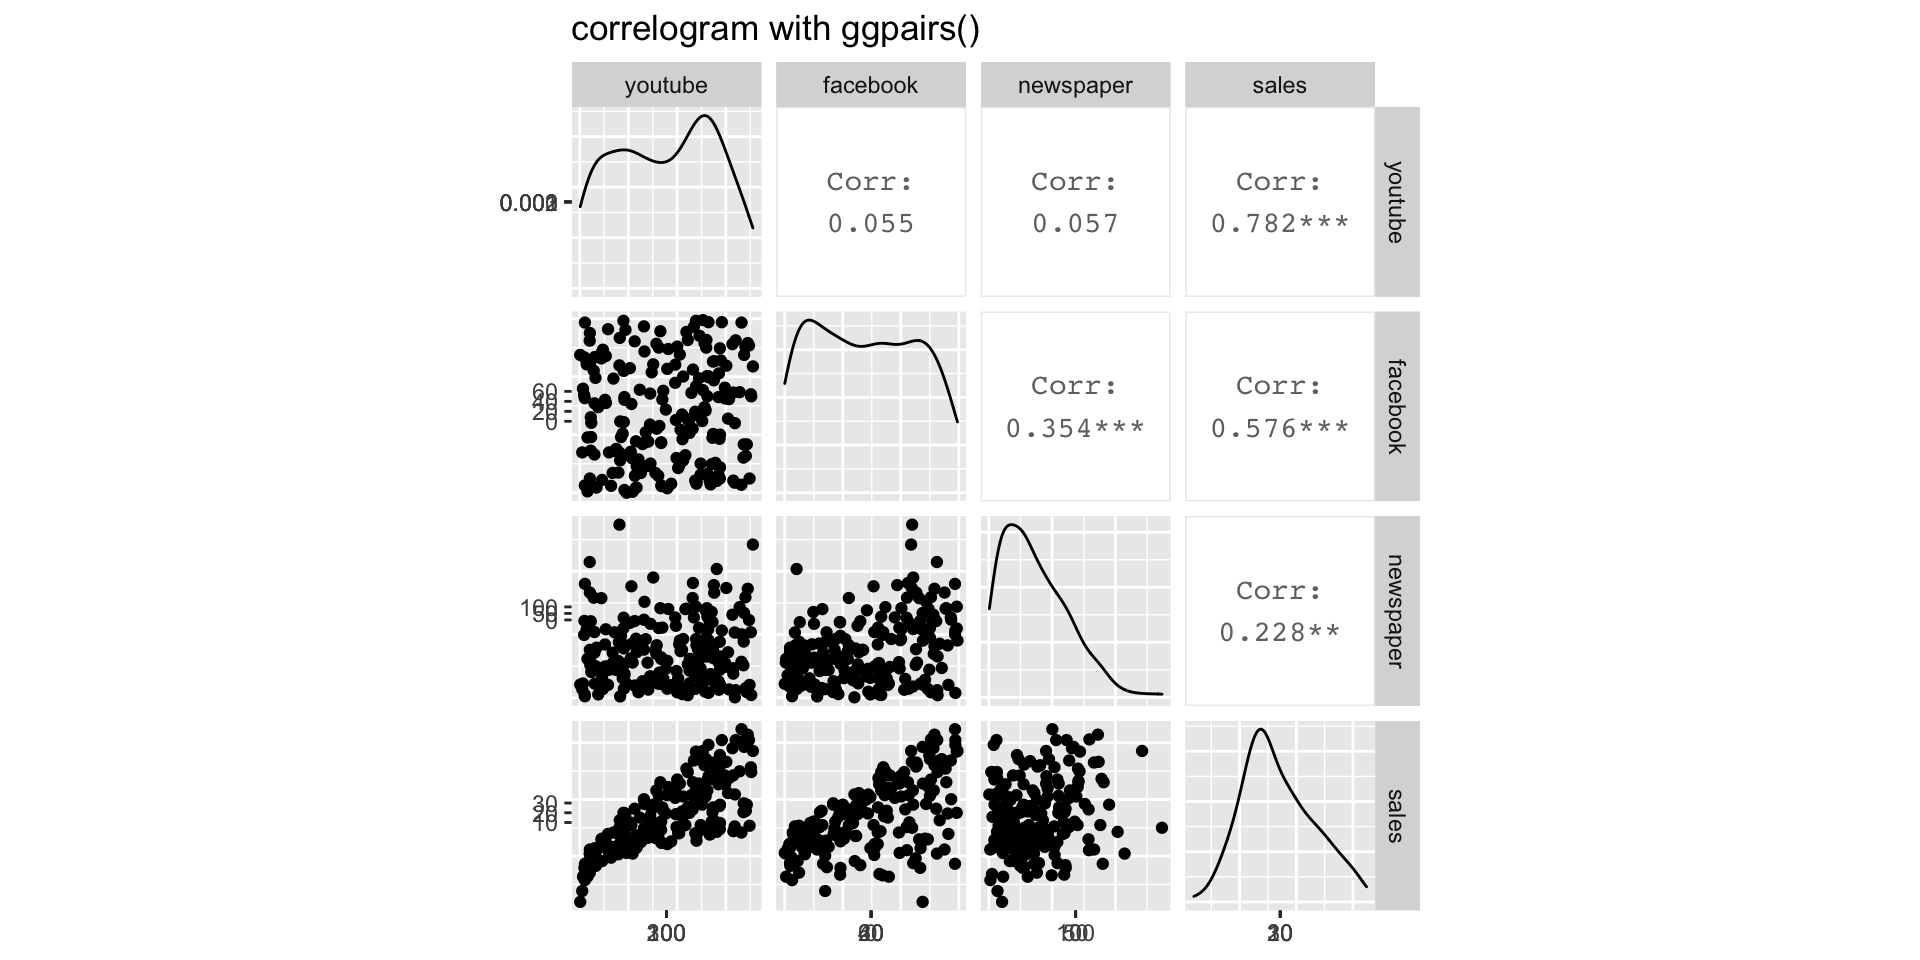
\includegraphics{figure/unnamed-chunk-27-1} \end{center}

\begin{itemize}
\tightlist
\item
  The term \(corr\) is the Pearson product-moment correlation coefficient (\(r\)).
\item
  It is a measure of the \textbf{linear} correlation of two variables.
\item
  It is a number that ranges from -1 to 0 to +1, representing th strength of the linear relationship between the variables.
\item
  An \(r\) value of \(+1\) denotes a perfect \textbf{linear} positive relationship between two variables.
\item
  An \(r\) value of \(-1\) denotes a perfect \textbf{linear} negative relationship between two variables, which indicates an inverse relationship between two variables: as one variable gets larger, the other gets smaller.
\item
  An \(r\) value of 0 means no \textbf{linear} relationship is present between the two variables (There can be a non-linear relationship.)
\end{itemize}

\hypertarget{simple-linear-regression}{%
\section{Simple Linear Regression}\label{simple-linear-regression}}

\begin{itemize}
\item
  The most elementary regression model is called \textbf{simple linear regression}.
\item
  The variable to be predicted is called the \emph{dependent variable} an is denoted by \(y\).
\item
  The \emph{predictor} is called the \emph{independent variable} or \emph{explanatory variable} and is denoted by \(x\)
\item
  In simple \emph{linear} regression analysis, only a strait-line relationship between two variables is examined.
\end{itemize}

\begin{Shaded}
\begin{Highlighting}[]
\CommentTok{\#lm(y \textasciitilde{} x)}
\NormalTok{reg }\OtherTok{\textless{}{-}} \FunctionTok{lm}\NormalTok{(sales }\SpecialCharTok{\textasciitilde{}}\NormalTok{ facebook,  }\AttributeTok{data =}\NormalTok{ marketing)}

\NormalTok{reg}
\end{Highlighting}
\end{Shaded}

\begin{verbatim}
## 
## Call:
## lm(formula = sales ~ facebook, data = marketing)
## 
## Coefficients:
## (Intercept)     facebook  
##     11.1740       0.2025
\end{verbatim}

\begin{Shaded}
\begin{Highlighting}[]
\FunctionTok{summary}\NormalTok{(reg)}
\end{Highlighting}
\end{Shaded}

\begin{verbatim}
## 
## Call:
## lm(formula = sales ~ facebook, data = marketing)
## 
## Residuals:
##      Min       1Q   Median       3Q      Max 
## -18.8766  -2.5589   0.9248   3.3330   9.8173 
## 
## Coefficients:
##             Estimate Std. Error t value Pr(>|t|)    
## (Intercept) 11.17397    0.67548  16.542   <2e-16 ***
## facebook     0.20250    0.02041   9.921   <2e-16 ***
## ---
## Signif. codes:  0 '***' 0.001 '**' 0.01 '*' 0.05 '.' 0.1 ' ' 1
## 
## Residual standard error: 5.13 on 198 degrees of freedom
## Multiple R-squared:  0.332,  Adjusted R-squared:  0.3287 
## F-statistic: 98.42 on 1 and 198 DF,  p-value: < 2.2e-16
\end{verbatim}

\hypertarget{residual-analysis}{%
\subsection{Residual Analysis}\label{residual-analysis}}

\begin{Shaded}
\begin{Highlighting}[]
\FunctionTok{par}\NormalTok{(}\AttributeTok{mfrow =} \FunctionTok{c}\NormalTok{(}\DecValTok{2}\NormalTok{,}\DecValTok{2}\NormalTok{))}
\FunctionTok{plot}\NormalTok{(reg)}
\end{Highlighting}
\end{Shaded}

\begin{center}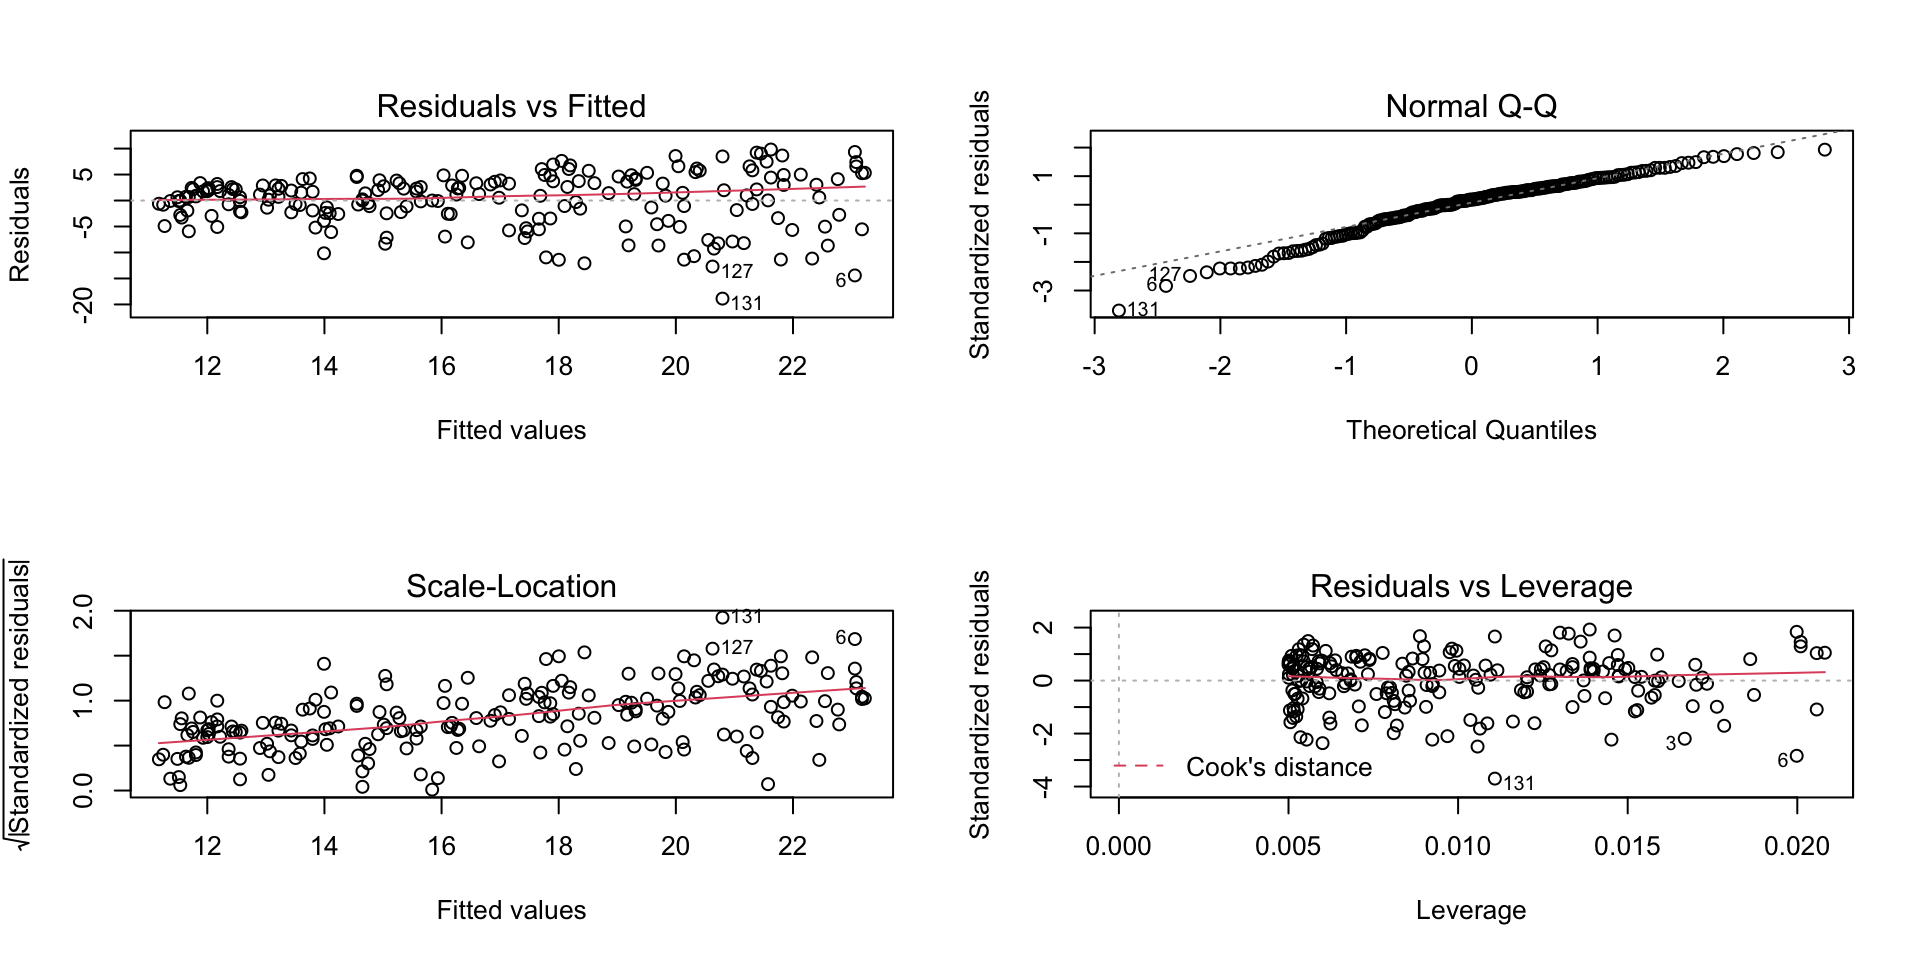
\includegraphics{figure/unnamed-chunk-29-1} \end{center}

\begin{itemize}
\item
  You want these plots to display random residuals (no patterns) that are uncorrelated and uniform.
\item
  Generally speaking, if you see patterns in the residuals, your model has a problem, and you might not be able to trust the results.
\item
  Heteroscedasticity produces a distinctive fan or cone shape in residual plots.
\item
  To check for heteroscedasticity, you need to assess the residuals by fitted value plots specifically.
\item
  Typically, the telltale pattern for heteroscedasticity is that as the fitted values increases, the variance of the residuals also increases.
\end{itemize}

Read more about residual analysis:

\begin{itemize}
\tightlist
\item
  Montgomery, D. C., Peck, E. A., \& Vining, G. G. (2012). Introduction to linear regression analysis (Vol. 821). John Wiley \& Sons.
\end{itemize}

\hypertarget{multiple-linear-regression}{%
\section{Multiple Linear Regression}\label{multiple-linear-regression}}

\begin{itemize}
\item
  Regression models with more than one independent variable can be explored by using multiple regression models.
\item
  We want to build a model for estimating sales based on the advertising budget invested in youtube, facebook and newspaper, as follow:
\end{itemize}

\[sales = \beta_0 + \beta_1*youtube + \beta_2*facebook + \beta_3*newspaper\]

You can compute the model coefficients in R as follow:

\begin{Shaded}
\begin{Highlighting}[]
\NormalTok{m\_reg }\OtherTok{\textless{}{-}} \FunctionTok{lm}\NormalTok{(sales }\SpecialCharTok{\textasciitilde{}}\NormalTok{ youtube }\SpecialCharTok{+}\NormalTok{ facebook }\SpecialCharTok{+}\NormalTok{ newspaper, }\AttributeTok{data =}\NormalTok{ marketing)}
\FunctionTok{summary}\NormalTok{(m\_reg)}
\end{Highlighting}
\end{Shaded}

\begin{verbatim}
## 
## Call:
## lm(formula = sales ~ youtube + facebook + newspaper, data = marketing)
## 
## Residuals:
##      Min       1Q   Median       3Q      Max 
## -10.5932  -1.0690   0.2902   1.4272   3.3951 
## 
## Coefficients:
##              Estimate Std. Error t value Pr(>|t|)    
## (Intercept)  3.526667   0.374290   9.422   <2e-16 ***
## youtube      0.045765   0.001395  32.809   <2e-16 ***
## facebook     0.188530   0.008611  21.893   <2e-16 ***
## newspaper   -0.001037   0.005871  -0.177     0.86    
## ---
## Signif. codes:  0 '***' 0.001 '**' 0.01 '*' 0.05 '.' 0.1 ' ' 1
## 
## Residual standard error: 2.023 on 196 degrees of freedom
## Multiple R-squared:  0.8972, Adjusted R-squared:  0.8956 
## F-statistic: 570.3 on 3 and 196 DF,  p-value: < 2.2e-16
\end{verbatim}

\hypertarget{how-to-test-if-your-linear-model-has-a-good-fit}{%
\subsection{How to test if your linear model has a good fit?}\label{how-to-test-if-your-linear-model-has-a-good-fit}}

\begin{itemize}
\item
  Most common value to check how good is your model is the coefficient of determinations or \(R^2\)
\item
  As we have seen in simple linear regression, the overall quality of the model can be assessed by examining the R-squared (\(R^2\)).
\item
  \(R^2=0.05602\) means that the model explains only 5\% of the data variability.
\item
  \(R^2\) represents the proportion of variance, in the outcome variable \(y\), that may be predicted by knowing the value of the \(x\) variables.
\item
  An \(R^2\) value close to 1 indicates that the model explains a large portion of the variance in the outcome variable.
\item
  The second one has an \(R^2\) of 0.89, and the model can explain \(89\%\) of the total variability.
\item
  In the regression summary output notice that there's two different \(R^2\), one multiple and one adjusted.
\item
  One problem with this \(R^2\) is that it will always increase when more variables are added to the model, even if those variables are only weakly associated with the response (i.e.~these variables don't add anything to your predictions)
\item
  For this reason, the \textbf{adjusted} \(R^2\) is probably better to look at if you are adding more than one variable to the model, since it only increases if it reduces the overall error of the predictions.
\item
  The adjustment in the \textbf{Adjusted R Square} value in the summary output is a correction for the number of x variables included in the prediction model.
\end{itemize}

\textbf{NOTE}

\emph{In our example, with youtube, newspaper and facebook predictor variables, the adjusted} \(R^2 = 0.89\), \emph{meaning that ``89\% of the variance in the measure of sales can be predicted by youtube, newspaper and facebook advertising budgets.}

\emph{This model is better than the simple linear model with only facebook, which had an adjusted} \(R^2\) \emph{of 0.05.}

\hypertarget{dont-forget-to-look-at-the-residuals}{%
\subsection{Don't forget to look at the residuals}\label{dont-forget-to-look-at-the-residuals}}

\begin{itemize}
\item
  You can have a pretty good \(R^2\) in your model, but let's not rush to conclusions here.
\item
  Ideally, when you plot the residuals, they should look random. Otherwise, it means that maybe there is a hidden pattern that the linear model is not considering.
\end{itemize}

\begin{Shaded}
\begin{Highlighting}[]
\FunctionTok{par}\NormalTok{(}\AttributeTok{mfrow =} \FunctionTok{c}\NormalTok{(}\DecValTok{2}\NormalTok{,}\DecValTok{2}\NormalTok{))}
\FunctionTok{plot}\NormalTok{(m\_reg)}
\end{Highlighting}
\end{Shaded}

\begin{center}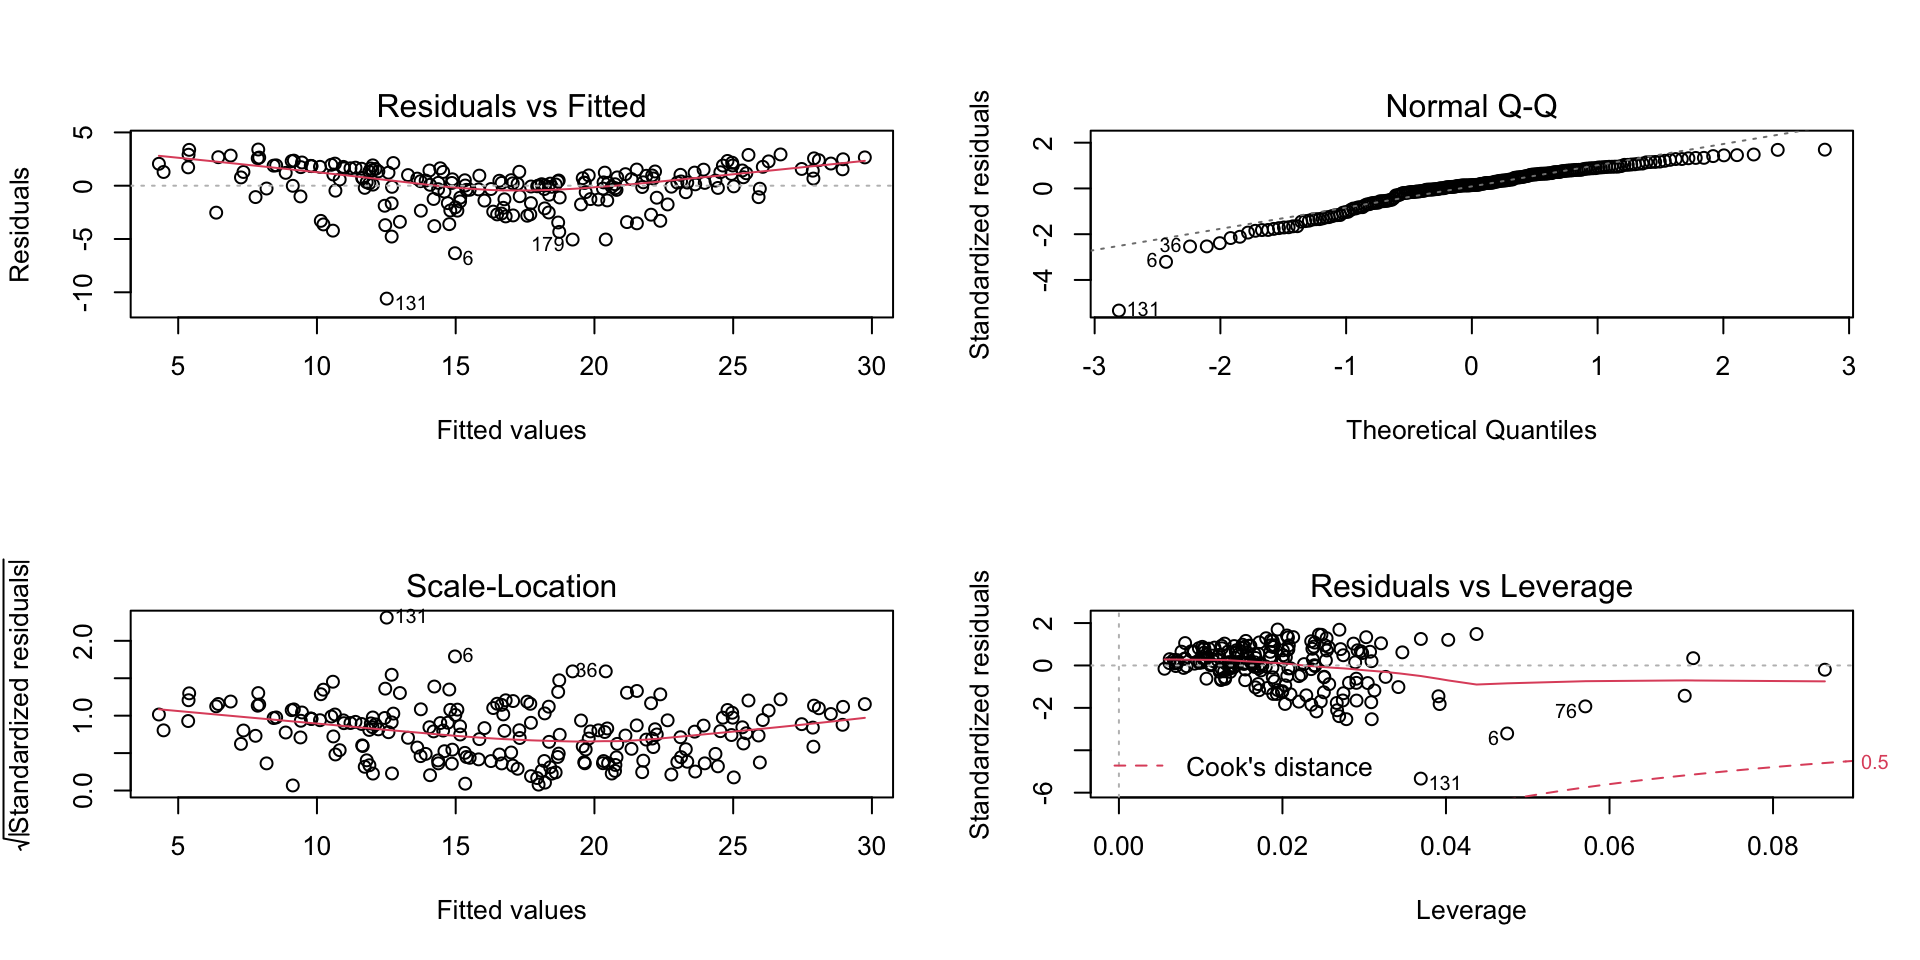
\includegraphics{figure/unnamed-chunk-31-1} \end{center}

\hypertarget{prediction-for-new-data-set}{%
\section{Prediction for new data set}\label{prediction-for-new-data-set}}

\begin{itemize}
\tightlist
\item
  Using the above model, we can predict the sales for a new advertising budget.
\end{itemize}

\begin{Shaded}
\begin{Highlighting}[]
\NormalTok{new.budget }\OtherTok{\textless{}{-}} \FunctionTok{data.frame}\NormalTok{(}
  \AttributeTok{youtube =} \FunctionTok{c}\NormalTok{(}\DecValTok{150}\NormalTok{, }\DecValTok{200}\NormalTok{, }\DecValTok{100}\NormalTok{),}
  \AttributeTok{facebook =} \FunctionTok{c}\NormalTok{( }\DecValTok{150}\NormalTok{, }\DecValTok{100}\NormalTok{, }\DecValTok{200}\NormalTok{),}
  \AttributeTok{newspaper =} \FunctionTok{c}\NormalTok{(}\DecValTok{0}\NormalTok{,}\DecValTok{0}\NormalTok{,}\DecValTok{0}\NormalTok{)}
\NormalTok{)}
\NormalTok{new.budget}
\end{Highlighting}
\end{Shaded}

\begin{verbatim}
##   youtube facebook newspaper
## 1     150      150         0
## 2     200      100         0
## 3     100      200         0
\end{verbatim}

\begin{Shaded}
\begin{Highlighting}[]
\FunctionTok{predict}\NormalTok{(m\_reg, new.budget)}
\end{Highlighting}
\end{Shaded}

\begin{verbatim}
##        1        2        3 
## 38.67087 31.53260 45.80914
\end{verbatim}

\textbf{Simple Linear regression}

\begin{Shaded}
\begin{Highlighting}[]
\NormalTok{new.facebook }\OtherTok{\textless{}{-}} \FunctionTok{data.frame}\NormalTok{(}
  \AttributeTok{facebook =} \FunctionTok{c}\NormalTok{(}\DecValTok{50}\NormalTok{, }\DecValTok{100}\NormalTok{, }\DecValTok{200}\NormalTok{)}
\NormalTok{)}

\FunctionTok{predict}\NormalTok{(reg, new.facebook)}
\end{Highlighting}
\end{Shaded}

\begin{verbatim}
##        1        2        3 
## 21.29875 31.42354 51.67312
\end{verbatim}

\newpage

\hypertarget{references-1}{%
\section{References}\label{references-1}}

\url{https://www.scribbr.com/statistics/linear-regression-in-r/}

\url{https://statisticsbyjim.com/regression/heteroscedasticity-regression/}

\newpage

hypothesis testing part

\url{http://www.sthda.com/english/articles/40-regression-analysis/168-multiple-linear-regression-in-r/}

\hypertarget{mtcars}{%
\chapter{mtcars}\label{mtcars}}

Cars Dataset: \url{https://www.rpubs.com/dksmith01/cars}

mtcars descriptive analysis: \url{https://rstudio-pubs-static.s3.amazonaws.com/481654_883a4b47c9b244d4859dd1db235f0165.html}

mtcars: regression analysis: \url{https://rstudio-pubs-static.s3.amazonaws.com/156794_e6ddaf8ca4ac4c2882a91dfa2ca8e3e8.html}

ANOVA: \url{https://medium.com/humansystemsdata/anova-with-mtcars-54dd6344c4e1}

two way anova: \url{https://www.geeksforgeeks.org/anova-test-in-r-programming/}

chisquare : \url{https://rpubs.com/daheza/assignment3}

\url{https://datascienceplus.com/chi-squared-test-in-r/}

descriptive statistics: \url{http://www.sthda.com/english/wiki/r-built-in-data-sets}

\url{http://www.sthda.com/english/wiki/r-built-in-data-sets}

explore mtcars: \url{https://cran.r-project.org/web/packages/explore/vignettes/explore_mtcars.html}

descrpive statistics: \url{https://rpubs.com/rpubsNovice/459602}

mpg: \url{https://www.sandicliffe.co.uk/blog/what-is-mpg\#}:\textasciitilde:text=MPG\%20is\%20an\%20abbreviation\%20for,a\%20car\%20or\%20commercial\%20vehicle.\&text=If\%20one\%20model\%20has\%20fuel,the\%20same\%20amount\%20of\%20fuel.

horseower: \url{https://www.quora.com/Why-does-horsepower-matter-Does-it-mean-better-MPG-or-something}

t-test and Chi Squared: \url{https://rpubs.com/daheza/assignment3}

code mtcars data : \url{http://psych.colorado.edu/~lharvey/P4165/P4165_2018_1_Spring/Material_2018_Spring_PSYC4165/Class_Handout_pdfs_2018_Spring_PSYC4165/R\%20guide_JMS\%20Revised_1_11_18.pdf}

page 15

  \bibliography{book.bib,packages.bib}

\end{document}
